\section{VỊ TRÍ TƯƠNG ĐỐI GIỮA HAI ĐƯỜNG THẲNG. GÓC VÀ KHOẢNG CÁCH}
\subsection{Tóm tắt lý thuyết}
\subsubsection{Vị trí tương đối giữa hai đường thẳng}
	Trên mặt phẳng tọa độ, xét hai đường thẳng $\Delta_1 \colon a_1 x+b_1 y+c_1=0$ và $\Delta_2 \colon a_2 x+b_2 y+c_2=0$.\\
	Khi đó, tọa độ giao điểm (nếu có) của $\Delta_1$ và $\Delta_2$ là nghiệm của hệ phương trình
	$$\heva{&a_1 x+b_1 y+c_1=0\\&a_2 x+b_2 y+c_2=0}\qquad(*)$$
	\begin{itemize}
		\item $\Delta_1$ cắt $\Delta_2$ tại $M(x_0;y_0)$ khi và chỉ khi hệ $(*)$ có nghiệm duy nhất $(x_0;y_0)$.
		\item $\Delta_1$ song song với $\Delta_2$ khi và chỉ khi $(*)$ vô nghiệm.
		\item $\Delta_1$ trùng $\Delta_2$ khi và chỉ khi hệ $(*)$ có vô số nghiệm.
	\end{itemize}
	\begin{note}
			Dựa vào các véc-tơ chỉ phương $\overrightarrow{u_1}$, $\overrightarrow{u_2}$ hoặc các véc-tơ pháp tuyến $\overrightarrow{n_1}$, $\overrightarrow{n_2}$ của $\Delta_1$, $\Delta_2$ ta có
		\begin{itemize}
			\item $\Delta_1$ và $\Delta_2$ song song hoặc trùng nhau $\Leftrightarrow \overrightarrow{u_1}$ và $\overrightarrow{u_2}$ cùng phương $\Leftrightarrow \overrightarrow{n_1}$ và $\overrightarrow{n_2}$ cùng phương.
			\begin{center}
				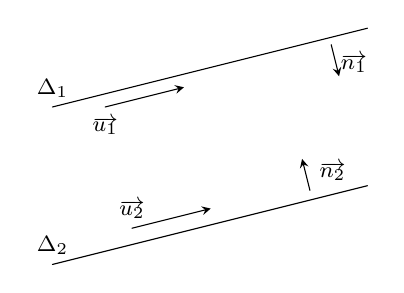
\begin{tikzpicture}[scale=1, font=\footnotesize, line join=round, line cap=round, >=stealth]
					\draw (0,0) node[above]{$\Delta_2$}
					--++(4,1);
					\draw (0,2) node[above]{$\Delta_1$}
					--++(4,1);
					\draw[->] (1.01,0.46) node[above]{$\overrightarrow{u_2}$}--++(1,0.25);
					\draw[->] (0.67,2) node[below]{$\overrightarrow{u_1}$}--++(1,0.25);
					\draw[->] (3.54,2.79) node[below right]{$\overrightarrow{n_1}$}--++(0.1,-0.4);
					\draw[->] (3.27,0.94) node[above right]{$\overrightarrow{n_2}$}--++(-0.1,0.4);
				\end{tikzpicture}	
			\end{center}
			\item $\Delta_1$ và $\Delta_2$ cắt nhau $\Leftrightarrow \overrightarrow{u_1}$ và $\overrightarrow{u_2}$ không cùng phương $\Leftrightarrow \overrightarrow{n_1}$ và $\overrightarrow{n_2}$ không cùng phương.
			\begin{center}
				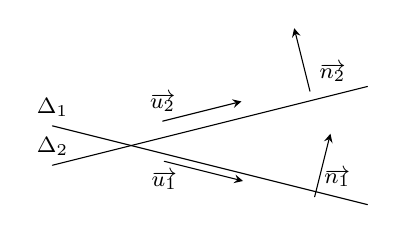
\begin{tikzpicture}[scale=1, font=\footnotesize, line join=round, line cap=round, >=stealth]
					\draw (0,0) node[above]{$\Delta_2$}
					--++(4,1);
					\draw[->] (1.4,0.56) node[above]{$\overrightarrow{u_2}$}--++(1,0.25);
					\draw[->] (3.27,0.94) node[above right]{$\overrightarrow{n_2}$}--++(-0.2,0.8);
					\draw (0,0.5) node[above]{$\Delta_1$}
					--++(4,-1);
					\draw[->] (1.42,0.05) node[below]{$\overrightarrow{u_1}$}--++(1,-0.25);
					\draw[->] (3.33,-0.4) node[above right]{$\overrightarrow{n_1}$}--++(0.2,0.8);
				\end{tikzpicture}	
			\end{center}
		\end{itemize}
	\end{note}
\subsubsection{Góc giữa hai đường thẳng}
	Hai đường thẳng cắt nhau tạo thành bốn góc, số đo của góc không tù được gọi là số đo góc (hay đơn giản là góc) giữa hai đường thẳng.\\
	Góc giữa hai đường thẳng song song hoặc trùng nhau được quy ước bằng $0^\circ$.\\
	Cho hai đường thẳng $\Delta_1\colon a_1 x+b_1y+c_1=0$ và $\Delta_2 \colon a_2 x+b_2y+c_2=0$, với các véc-tơ pháp tuyến $\overrightarrow{n_1}=(a_1;b_1)$ và $\overrightarrow{n_2}=(a_2;b_2)$ tương ứng. Khi đó, góc $\varphi$ giữa hai đường thẳng đó được xác định thông qua công thức $$\cos\varphi=\left|\cos\left(\overrightarrow{n_1},\overrightarrow{n_2}\right)\right|=\dfrac{\left|\overrightarrow{n_1}\cdot \overrightarrow{n_2}\right|}{\left|\overrightarrow{n_1}\right|\cdot \left|\overrightarrow{n_2}\right|}=\dfrac{\left|a_1a_2+b_1b_2\right|}{\sqrt{a_1^2+b_1^2}\cdot \sqrt{a_2^2+b_2^2}}.$$
\subsubsection{Khoảng cách từ một điểm đến một đường thẳng}	
	Cho điểm $M(x_0;y_0)$ và đường thẳng $\Delta \colon ax+by+c=0$. Khoảng cách từ điểm $M$ đến đường thẳng $\Delta$, ký hiệu là $\mathrm{\,d}(M,\Delta)$, được tính bởi công thức $$\mathrm{\,d}(M,\Delta)=\dfrac{\left|ax_0+by_0+c\right|}{\sqrt{a^2+b^2}}.$$
\subsection{Các dạng toán}
	\begin{dang}{Xét vị trí tương đối giữa hai đường thẳng}
		\textbf{Phương pháp chung}
		\begin{itemize}
			\item [$\bullet$] Xét hệ phương trình tạo bởi hai đường thẳng.
			\item [$\bullet$] Tìm số nghiệm của hệ phương trình, từ đó kết luận vị trí tương đối giữa hai đường thẳng.
		\end{itemize}
	\begin{note}
		Ta có thể xét theo trình tự: \begin{itemize}
			\item Kiểm tra hai véc-tơ chỉ phương (hoặc hai véc-tơ pháp tuyến) của hai đường thẳng có cùng phương hay không.
			\item Nếu chúng không cùng phương $\Rightarrow $ hai đường thẳng cắt nhau. Nếu chúng cùng phương, kiểm tra một điểm bất kỳ thuộc đường thẳng này có thuộc đường thẳng kia hay không.
		\end{itemize}
	\end{note}
	\end{dang}
	\viduminhhoa
	\setcounter{vd}{0}
	\begin{vd}%[0H3Y1-3]
		Trong mặt phẳng tọa độ $Oxy$, xét vị trí tương đối giữa đường thẳng $\Delta \colon x-3y+1=0$ và mỗi đường thẳng $d_1 \colon x+y-2=0$ và $d_2 \colon -2x+6y+5=0$.
		\loigiai{
		\begin{itemize}
			\item Xét hệ phương trình $\heva{&x-3y+1=0\\&x+y-2=0}\Leftrightarrow \heva{&x=\dfrac{5}{4}\\&y=\dfrac{3}{4}}$ nên $\Delta$ và $d_1$ cắt nhau.
			\item Xét hệ phương trình $\heva{&x-3y+1=0\\&-2x+6y+5=0}$, hệ phương trình vô nghiệm nên $\Delta$ và $d_2$ song song với nhau.
		\end{itemize}	
		}
	\end{vd}
	\begin{vd}%[0H3Y1-3]
		Trong mặt phẳng tọa độ $Oxy$, xét vị trí tương đối của hai đường thẳng $d \colon 3x-4y+1=0$ và $\Delta \colon \heva{&x=4t\\&y=1+3t}$.
		\loigiai{
		Đường thẳng $d$ đi qua $A(1;1)$ và có một véc-tơ pháp tuyến là $\overrightarrow{n}=(3;-4)$.\\
		Đường thẳng $\Delta$ đi qua $M(0;1)$ và nhận $\overrightarrow{u}=(4;3)$ làm véc-tơ chỉ phương, nên $\overrightarrow{n'}=(3;-4)$ là một véc-tơ pháp tuyến của $\Delta$.\\
		Vì $\overrightarrow{n}$, $\overrightarrow{n'}$ cùng phương nên $d$ và $\Delta$ song song hoặc trùng nhau. Mặt khác $M(0;1)\notin d$ nên $d \parallel \Delta$.
		}
	\end{vd}
	\begin{vd}%[0H3Y1-3]
		Trong mặt phẳng tọa độ $Oxy$ cho hai đường thẳng lần lượt có phương trình $\Delta_1 \colon 3x-2y+4=0$, $\Delta_2\colon 2x+y+5=0$. Tìm tọa độ giao điểm $I$ của hai đường thẳng $\Delta_1$ và $\Delta_2$.
		\loigiai{
			Tọa độ giao điểm $I$ của hai đường thẳng $\Delta_1$ và $\Delta_2$ là nghiệm của hệ phương trình
			$$\heva{&3x-2y+4=0\\&2x+y+5=0}\Leftrightarrow \heva{&x=-2\\&y=-1}\Rightarrow I(-2;-1).$$
		}
	\end{vd}
	\begin{vd}%[0H3B1-3]
		Đường thẳng $\Delta \colon 5x-y=10$ tạo với các trục tọa độ tam giác có diện tích bằng bao nhiêu?
		\loigiai{
		Tọa độ giao điểm $A$ của đường thẳng $\Delta$ và trục $Ox \colon y=0$ là nghiệm của hệ phương trình $\heva{&5x-y=10\\&y=0}\Leftrightarrow \heva{&x=2\\&y=0}\Rightarrow A(2;0)$.\\
		Tọa độ giao điểm $B$ của đường thẳng $\Delta$ và trục $Oy \colon x=0$ là nghiệm của hệ phương trình $\heva{&5x-y=10\\&x=0}\Leftrightarrow \heva{&x=0\\&y=-10}\Rightarrow B(0;-10)$.\\
		Diện tích tam giác $\triangle OAB$ là $S_{\triangle OAB}=\dfrac{1}{2} \cdot 2 \cdot 10=10$.
		}
	\end{vd}
	\begin{vd}%[0H3B1-3]
		Trong mặt phẳng tọa độ $Oxy$, hai đường thẳng $d_1 \colon mx+y-m-1=0$ và $d_2 \colon x+my-2=0$ song song với nhau khi và chỉ khi
		\loigiai{
			Hai đường thẳng $d_1$ và $d_2$ song song khi và chỉ khi\\
			$\dfrac{m}{1}=\dfrac{1}{m} \ne \dfrac{-1}{-2} \Leftrightarrow \heva{&m^2=1 \\& \hoac{&m \ne \dfrac{1}{2} \\& m \ne 2}}\Leftrightarrow m=\pm 1$.
		}
	\end{vd}
	\begin{vd}%[0H3B1-3]
		Trong mặt phẳng với hệ tọa độ $Oxy$, cho ba đường thẳng lần lượt có phương trình $d_1 \colon 5x-6y-4=0$, $d_2 \colon x+2y-4=0$, $d_3 \colon mx-(2m-1)y+9m-19=0$ ($m$ là tham số). Tìm tất cả các giá trị của tham số $m$ để ba đường thẳng đã cho cùng đi qua một điểm?
		\loigiai{
			Tọa độ giao điểm của $d_1$ và $d_2$ thỏa hệ $\heva{&5x-6y-4=0 \\& x+2y-4=0}\Leftrightarrow \heva{&x=2 \\& y=1.}$ Vậy $d_1;d_2$ cắt nhau tại $M(2;1)$.\\
			Để ba đường thẳng đã cho cùng đi qua một điểm thì $d_3$ qua $M(2;1)$ \\
			Hay $2m-(2m-1)+9m-19=0 \Leftrightarrow 9m-18=0 \Leftrightarrow m=2$.
		}
	\end{vd}
	\begin{vd}%[0H3B1-6]
		Trong mặt phẳng $Oxy$, cho $P(1;3)$, $Q(2;-1)$ và đường thẳng $d \colon x+y+2=0$. Tìm tọa độ giao điểm của đường thẳng $PQ$ và $d$.
		\loigiai{
			Ta có $\overrightarrow{PQ}=(1;-4) \Rightarrow \overrightarrow{n}_{PQ}=(4;1)$.\\
			Phương trình tổng quát đường thẳng $PQ \colon 4(x-1)+1(y-3)=0 \Leftrightarrow 4x+y-7=0$.\\
			Giao điểm của $PQ$ và $d$ có tọa độ là nghiệm của hệ phương trình $\heva{&4x+y-7=0 \\& x+y+2=0}\Leftrightarrow \heva{&x=3 \\& y=-5.}$
		}
	\end{vd}
	\baitaptl
	\setcounter{bt}{0}
	\begin{bt}%[Phạm Tuấn]%[0H3B1-2]
		Xét vị trí tương đối của cặp đường thẳng $d_1\colon 2x-y+2=0$ và $d_2\colon -4x+2y+1=0$. Tìm tọa độ giao điểm nếu chúng cắt nhau.
		\dapso{Hai đường thẳng $d_1$, $d_2$ song song}
		\loigiai{Ta có $\dfrac{2}{-4}=\dfrac{-1}{2}\ne\dfrac{2}{1}$ nên $d_1\parallel d_2$.
		}
	\end{bt}
	
	\begin{bt}%[Phạm Tuấn]%[0H3B1-2]
		Xét vị trí tương đối của cặp đường thẳng $d_1\colon x=2$ và $d_2\colon x+2y-4=0$. Tìm tọa độ giao điểm nếu chúng cắt nhau.
		\dapso{Hai đường thẳng $d_1$, $d_2$ cắt nhau tại điểm $M(2;1)$}
		\loigiai{Ta có $\dfrac{1}{1}\ne\dfrac{0}{2}$ nên $d_1$ và $d_2$ cắt nhau.\\
			Khi đó tọa độ giao điểm là nghiệm của hệ $\heva{&x=2\\&x+2y-4=0}\Leftrightarrow\heva{&x=2\\&y=1.}$\\
			Vậy tọa độ giao điểm là $\left(2;1\right)$.
		}
	\end{bt}
	
	\begin{bt}%[Phạm Tuấn]%[0H3B1-2]
		Xét vị trí tương đối của cặp đường thẳng $d_1\colon \heva{&x=5+t\\&y=-3+2t}$ và $d_2\colon \heva{&x=4+t'\\&y=-3+3t'}$. Tìm tọa độ giao điểm nếu chúng cắt nhau.
		\dapso{Hai đường thẳng $d_1$ và $d_2$ cắt nhau tại điểm $M(2;-9)$}
		\loigiai{
			Xét hệ phương trình $$\heva{&5+t=4+t'\\&-3+2t=-3+3t'}\Leftrightarrow\heva{&t-t'=-1\\&2t-3t'=0}\Leftrightarrow \heva{&t=-3\\&t'=-2.}$$
			Do hệ có nghiệm duy nhất nên $d_1$ cắt $d_2$ và tọa độ giao điểm là $\left(2;-9\right)$.
		}
	\end{bt}
	
	\begin{bt}%[Phạm Tuấn]%[0H3B1-2]
		Cho hai đường thẳng $d\colon mx-2y+1=0$ và $\Delta\colon 2x+y-3=0$. Tìm tất cả các giá trị của $m$ để hai đường thẳng $d$ và $\Delta$
		\begin{enumerate}
			\item Cắt nhau.		\dapso{$m\neq -4$}
			\item Song song.	\dapso{$m=-4$}
			\item Trùng nhau.	\dapso{không tồn tại $m$}	
		\end{enumerate}
		\loigiai
		{Xét hệ phương trình $\heva{&mx-2y+1=0\\&2x+y-3=0} \quad (I)$.
			\begin{enumerate}
				\item Hai đường thẳng $d$ và $\Delta$ cắt nhau khi và chỉ khi hệ $(I)$ có nghiệm duy nhất $$\Leftrightarrow \dfrac{m}{2}\ne \dfrac{-2}{1} \Leftrightarrow m\neq -4.$$
				\item Hai đường thẳng $d$ và $\Delta$ song song khi và chỉ khi hệ $(I)$ vô nghiệm
				$$\Leftrightarrow \dfrac{m}{2}=\dfrac{-2}{1}\ne \dfrac{-1}{3} \Leftrightarrow m+4=0 \Leftrightarrow m=-4.$$
				\item Do $\dfrac{-2}{1}\ne \dfrac{-1}{3}$ nên hệ $(I)$ không thể có vô số nghiệm. Do đó $d$ và $\Delta$ không thể trùng nhau.
		\end{enumerate}}
	\end{bt}
	
	\begin{bt}%[Phạm Tuấn]%[0H3B1-2]
		Cho hai đường thẳng $d\colon 2mx+(m-1)y-2=0$ và $\Delta\colon (m+2)x+(2m+1)y-(m+2)=0$. Tìm tất cả các giá trị của $m$ để hai đường thẳng $d$ và $\Delta$
		\begin{enumerate}
			\item Cắt nhau.		\dapso{mọi $m\in\mathbb{R}$}
			\item Song song.	\dapso{không tồn tại $m$}
			\item Trùng nhau.	\dapso{không tồn tại $m$}	
		\end{enumerate}
		\loigiai
		{Xét hệ phương trình $\heva{&2mx+(m-1)y-2=0\\&(m+2)x+(2m+1)y-(m+2)=0}$, có
			$$D=\begin{vmatrix}
				2m&m-1\\m+2&2m+1
			\end{vmatrix}= 2m(2m+1)-(m-1)(m+2)=3m^2+m+2 = 2m^2+\left(m+\dfrac{1}{2}\right)^2+\dfrac{7}{4}>0, \forall m.$$
			Vậy hệ phương trình luôn có nghiệm duy nhất, do đó hai đường thẳng $d$, $\Delta$ luôn cắt nhau với mọi $m$.}
	\end{bt}
	
	\begin{bt}%[Phạm Tuấn]%[0H3B1-2]
		Cho hai đường thẳng $d\colon (m-2)x+(m-6)y+(m-1)=0$ và $\Delta\colon (m-4)x+(2m-3)y+m-5=0$. Tìm tất cả các giá trị của $m$ để hai đường thẳng $d$ và $\Delta$
		\begin{enumerate}
			\item Cắt nhau.		\dapso{$m\neq 3$, $m\neq -6$}
			\item Song song.	\dapso{$m=-6$}
			\item Trùng nhau.	\dapso{$m=3$}	
		\end{enumerate}
		\loigiai{
			Xét hệ phương trình $\heva{&(m-2)x+(m-6)y+(m-1)=0\\&(m-4)x+(2m-3)y+m-5=0} \quad (I)$, có\\
			$D=\begin{vmatrix}
				m-2&m-6\\m-4&2m-3
			\end{vmatrix}= (m-2)(2m-3)-(m-6)(m-4)=(m-3)(m+6)$.\\
			$D_x=\begin{vmatrix}
				1-m&m-6\\5-m&2m-3
			\end{vmatrix}= (1-m)(2m-3)-(m-6)(5-m)=-(m-3)(m+9)$.\\
			$D_y=\begin{vmatrix}
				m-2&1-m\\m-4&5-m
			\end{vmatrix}=(m-2)(5-m)-(1-m)(m-4)=2(m-3)$.
			\begin{enumerate}
				\item Hai đường thẳng $d$ và $\Delta$ cắt nhau khi và chỉ khi hệ $(I)$ có nghiệm duy nhất $$\Leftrightarrow D=(m-3)(m+6)\neq 0 \Leftrightarrow \heva{&m\neq 3\\&m\neq -6.}$$
				Với $m=3$ ta có $D=D_x=D_y=0$ nên hệ $(I)$ có vô số nghiệm.\\
				Với $m=-6$ ta có $D=0$, $D_x=27$, $D_y=-18$ nên hệ $(I)$ vô nghiệm.
				\item Hai đường thẳng $d$ và $\Delta$ song song khi và chỉ khi hệ $(I)$ vô nghiệm
				$\Leftrightarrow m=-6$.
				\item Hai đường thẳng $d$ và $\Delta$ trùng nhau khi và chỉ khi hệ $(I)$ có vô số nghiệm $\Leftrightarrow m=3$.
			\end{enumerate}
		}
	\end{bt}
	\begin{bt}%[Phạm Tuấn]%[0H3B1-2]
		Cho điểm $A(2;1)$ và hai đường thẳng $d_1\colon 3x-2y+10=0$, $d_2\colon 4x+3y-7=0$. Viết phương trình đường thẳng $d$ qua $A$ và giao điểm của hai đường thẳng $d_1$, $d_2$.
		\dapso{$22x+25y-69=0$}
		\loigiai
		{Tọa độ giao điểm của hai đường thẳng $d_1$ và $d_2$ là nghiệm của hệ phương trình 
			$$\heva{&3x-2y+10=0\\&4x+3y-7=0} \Leftrightarrow \heva{&x=-\dfrac{16}{17}\\&y=\dfrac{61}{17}.}$$
			Suy ra giao điểm của $d_1$ và $d_2$ là điểm $M\left(-\dfrac{16}{17};\dfrac{61}{17}\right)$.\\
			Đường thẳng $d$ đi qua hai điểm $A$, $M$ nên có véc-tơ chỉ phương $\overrightarrow{AM}=\left(-\dfrac{50}{17};\dfrac{44}{17}\right)$, ta chọn véc-tơ pháp tuyến của đường thẳng $d$ là $\overrightarrow{n}=\left(22;25\right)$. Vậy phương trình đường thẳng $d$ là
			$$22(x-2)+25(y-1)=0 \Leftrightarrow 22x+25y-69=0.$$}
	\end{bt}
	
	\begin{bt}%[Phạm Tuấn]%[0H3B1-2]
		Tìm tất cả các giá trị của $m$ để ba đường thẳng $d_1\colon x+y+1=0$, $d_2\colon 3x+5y=-1$, $d_3\colon (m+1)x-my=3m+4$ đồng quy.
		\dapso{$m=-1$}
		\loigiai
		{Xét hệ phương trình $\heva{&x+y+1=0\\&3x+5y=-1}\Leftrightarrow \heva{&x=-2\\&y=1.}$\\
			Do đó hai đường thẳng $d_1$, $d_2$ cắt nhau tại điểm $M(-2;1)$.\\
			Ba đường thẳng $d_1$, $d_2$, $d_3$ đồng quy khi và chỉ khi đường thẳng $d_3$ đi qua $M$ 
			$$\Leftrightarrow -2\left(m+1\right)-m=3m+4 \Leftrightarrow 6m=-6 \Leftrightarrow m=-1.$$
			Khi đó đường thẳng $d_3\colon y=1$.}
	\end{bt}
	
	\begin{bt}%[Phạm Tuấn]%[0H3B1-2]
		Viết phương trình đường thẳng $d_2$ đi qua $A\left(1;1\right)$ và song song với đường thẳng $d_1\colon 2x-y+1=0$.
		\dapso{$2x+y-3=0$}
		\loigiai{Do $d_2\parallel d_1$ nên một véc-tơ pháp tuyến của $d_2$ là $\overrightarrow{n}=\left(2;1\right)$.\\
			Vậy phương trình đường thẳng $d_2$ là $2\left(x-1\right)+1\left(y-1\right)=0\Leftrightarrow 2x+y-3=0$.
		}
	\end{bt}
	\begin{bt}%[Phạm Tuấn]%[0H3B1-2]
		Cho ba đường thẳng $d_1\colon 3x-5y+2=0$, $d_2\colon 5x-2y+4=0$ và $d_3\colon 2x-y+4=0$. Viết phương trình đường thẳng $d$ qua giao điểm của hai đường thẳng $d_1$, $d_2$ và song song với đường thẳng $d_3$.
		\dapso{$2x-y+\dfrac{30}{19}=0$}
		\loigiai
		{Tọa độ giao điểm của hai đường thẳng $d_1$ và $d_2$ là nghiệm của hệ phương trình 
			$$\heva{&3x-5y+2=0\\&5x-2y+4=0} \Leftrightarrow \heva{&x=-\dfrac{16}{19}\\&y=-\dfrac{2}{19}.}$$
			Suy ra giao điểm của $d_1$ và $d_2$ là điểm $M\left(-\dfrac{16}{19};-\dfrac{2}{19}\right)$.\\
			Đường thẳng $d$ qua $M$ và song song với đường thẳng $d_3$ nên có phương trình
			$$2\left(x+\dfrac{16}{19}\right)-\left(y+\dfrac{2}{19}\right)=0 \Leftrightarrow 2x-y+\dfrac{30}{19}=0 \text{ (thỏa mãn)}.$$}
	\end{bt}
	\begin{bt}%[Phạm Tuấn]%[0H3B1-2]
		Cho ba đường thẳng $d_1\colon x-2y+5=0$, $d_2\colon 2x+3y-4=0$ và $d_3\colon 4x-3y+5=0$. Viết phương trình đường thẳng $d$ qua giao điểm của hai đường thẳng $d_1$, $d_2$ và vuông góc với đường thẳng $d_3$.
		\dapso{$3x+4y-5=0$}
		\loigiai
		{Tọa độ giao điểm của hai đường thẳng $d_1$ và $d_2$ là nghiệm của hệ phương trình 
			$$\heva{&x-2y+5=0\\&2x+3y-4=0} \Leftrightarrow \heva{&x=-1\\&y=2.}$$
			Suy ra giao điểm của $d_1$ và $d_2$ là điểm $M\left(-1;2\right)$.\\
			Đường thẳng $d_3$ có véc-tơ pháp tuyến $\overrightarrow{n_3}=(4;-3)$.\\
			Đường thẳng $d$ qua $M$ và vuông góc với đường thẳng $d_3$ nên có véc-tơ pháp tuyến $\overrightarrow{n}=(3;4)$, phương trình đường thẳng $d$ là
			$$3\left(x+1\right)+4\left(y-2\right)=0 \Leftrightarrow 3x+4y-5=0.$$}
	\end{bt}
	
	\begin{bt}%[Phạm Tuấn]%[0H3K1-2]
		Cho tam giác $ABC$ có $A(0;-1)$, $B(2;-3)$, $C(2;0)$.
		\begin{enumerate}
			\item Viết phương trình các đường trung tuyến của tam giác.
			\dapso{$AM\colon x+4y+4=0$, $BN\colon 5x+2y-4=0$, $CP\colon 2x-y-4=0$}
			\item Viết phương trình các đường cao của tam giác.
			\dapso{$AD\colon y+1=0$, $BE\colon 2x+y-1=0$, $CF\colon x-y-2=0$}
			\item Viết phương trình các đường trung trực của tam giác $ABC$.
			\dapso{$d_M\colon y+\dfrac{3}{2}=0$, $d_N\colon 2x+y-\dfrac{3}{2}=0$, $d_P\colon x-y-3=0$}
		\end{enumerate}
		\loigiai{
			Tam giác $ABC$ có $A(0;-1)$, $B(2;-3)$, $C(2;0)$. Gọi $M$, $N$, $P$ lần lượt là trung điểm các cạnh $BC$, $CA$, $AB$. Khi đó $M\left(2;-\dfrac{3}{2}\right)$, $N\left(1;-\dfrac{1}{2}\right)$, $P\left(1;-2\right)$.
			\begin{enumerate}
				\item Đường trung tuyến $AM$ có véc-tơ chỉ phương $\overrightarrow{AM}=\left(2;-\dfrac{1}{2}\right)$ nên có véc-tơ pháp tuyến $\overrightarrow{n}_{AM}=(1;4)$. Vậy phương trình $AM$ là
				$$x+4(y+1)=0 \Leftrightarrow x+4y+4=0.$$
				\immini
				{Đường trung tuyến $BN$ có véc-tơ chỉ phương $\overrightarrow{BN}=\left(-1;\dfrac{5}{2}\right)$ nên có véc-tơ pháp tuyến $\overrightarrow{n}_{BN}=(5;2)$. Vậy phương trình $BN$ là
					$$5(x-2)+2(y+3)=0 \Leftrightarrow 5x+2y-4=0.$$
					Đường trung tuyến $CP$ có véc-tơ chỉ phương $\overrightarrow{CP}=\left(-1;-2\right)$ nên có véc-tơ pháp tuyến $\overrightarrow{n}_{CP}=(2;-1)$. Vậy phương trình $CP$ là
					$$2(x-2)-y=0 \Leftrightarrow 2x-y-4=0.$$}
				{\begin{tikzpicture}[scale=1, font=\footnotesize,line join=round, line cap=round, >=stealth]
						\clip (-0.5,-1.5) rectangle (4.5,3.5);
						\coordinate (A) at (1,3);
						\coordinate (B) at (0,0);
						\coordinate (C) at (4,0);
						\coordinate (M) at ($(B)!1/2!(C)$);
						\coordinate (N) at ($(A)!1/2!(C)$);
						\coordinate (P) at ($(A)!1/2!(B)$);
						\draw (A)node[above]{$A$}--(B)node[below]{$B$}--(C)node[below]{$C$}--cycle;
						\draw (A)--(M)node[below]{$M$};
						\draw (B)--(N)node[above right]{$N$};
						\draw (C)--(P)node[above left]{$P$};
						\foreach \i in {A,B,C,M,N,P} \fill (\i) circle(1pt);
						\tkzMarkSegments[mark=||](B,M C,M)
						\tkzMarkSegments[mark=x](A,N C,N)
						\tkzMarkSegments[mark=|](A,P B,P)
				\end{tikzpicture}}
				\item Đường cao $AD$ qua $A$ và nhận véc-tơ $\overrightarrow{BC}=(0;3)$ làm véc-tơ pháp tuyến nên có phương trình $3(y+1)=0 \Leftrightarrow y+1=0$.
				\immini
				{Đường cao $BE$ qua $B$ và nhận véc-tơ $\overrightarrow{CA}=(-2;-1)$ làm véc-tơ pháp tuyến nên có phương trình $$-2(x-2)-1(y+3)=0 \Leftrightarrow 2x+y-1=0.$$
					Đường cao $CF$ qua $C$ và nhận véc-tơ $\overrightarrow{AB}=(2;-2)$ làm véc-tơ pháp tuyến nên có phương trình $$2(x-2)-2y=0 \Leftrightarrow x-y-2=0.$$}
				{\begin{tikzpicture}[scale=1, font=\footnotesize,line join=round, line cap=round, >=stealth]
						\clip (-0.5,-0.5) rectangle (4.5,3.5);
						\coordinate (A) at (1,3);
						\coordinate (B) at (0,0);
						\coordinate (C) at (4,0);
						\tkzDefPointBy[projection=onto B--C](A)\tkzGetPoint{D}
						\tkzDefPointBy[projection=onto A--C](B)\tkzGetPoint{E}
						\tkzDefPointBy[projection=onto A--B](C)\tkzGetPoint{F}
						\draw (A)node[above]{$A$}--(B)node[below]{$B$}--(C)node[below]{$C$}--cycle;
						\draw (A)--(D)node[below]{$D$};
						\draw (B)--(E)node[above right]{$E$};
						\draw (C)--(F)node[above left]{$F$};
						\foreach \i in {A,B,C,D,E,F} \fill (\i) circle(1pt);
						\tkzMarkRightAngles[size=0.15](A,D,C B,E,C C,F,B)
				\end{tikzpicture}}
				\item Đường trung trực $d_M$ của $BC$ qua $M$ và nhận véc-tơ $\overrightarrow{BC}=(0;3)$ làm véc-tơ pháp tuyến nên có phương trình $3\left(y+\dfrac{3}{2}\right)=0 \Leftrightarrow y+\dfrac{3}{2}=0$.\\
				\immini
				{Đường trung trực $d_N$ của $CA$ qua $N$ và nhận véc-tơ $\overrightarrow{CA}=(-2;-1)$ làm véc-tơ pháp tuyến nên có phương trình $$-2(x-1)-1\left(y+\dfrac{1}{2}\right)=0 \Leftrightarrow 2x+y-\dfrac{3}{2}=0.$$
					Đường trung trực $d_P$ của $AB$ qua $P$ và nhận véc-tơ $\overrightarrow{AB}=(2;-2)$ làm véc-tơ pháp tuyến nên có phương trình $$2(x-1)-2(y+2)=0 \Leftrightarrow x-y-3=0.$$}
				{\begin{tikzpicture}[scale=1, font=\footnotesize,line join=round, line cap=round, >=stealth]
						\clip (-0.8,-1.5) rectangle (4.5,3.5);
						\coordinate (A) at (1,3);
						\coordinate (B) at (0,0);
						\coordinate (C) at (4,0);
						\coordinate (M) at ($(B)!1/2!(C)$);
						\coordinate (N) at ($(A)!1/2!(C)$);
						\coordinate (P) at ($(A)!1/2!(B)$);
						\draw (A)node[above]{$A$}--(B)node[below]{$B$}--(C)node[below]{$C$}--cycle;
						\tkzCircumCenter(A,B,C)\tkzGetPoint{I}
					%	\draw (I)--(M) node[above]{$d_M$};
					%	\draw (I)--(N) node[above]{$d_N$};
					%	\draw (I)--(P) node[above]{$d_P$};
						\tkzDrawLines[add = 0.5 and 0.8](I,M)
						\tkzDrawLines[add = 0.5 and 0.8](I,N)
						\tkzDrawLines[add = 0.5 and 0.8](I,P)
						\node at (M)[below left]{$M$};
						\node at (N)[above]{$N$};
						\node at (P)[above left=-2pt]{$P$};
						\foreach \i in {A,B,C,M,N,P} \fill (\i) circle(1pt);
						\tkzMarkSegments[mark=||](B,M C,M)
						\tkzMarkSegments[mark=x](A,N C,N)
						\tkzMarkSegments[mark=|](A,P B,P)
				\end{tikzpicture}}
		\end{enumerate}
	}
	\end{bt}
	\begin{bt}%[Phạm Tuấn]%[0H3K1-2]
		Viết phương trình đường thẳng $d$ song song với đường thẳng $\Delta\colon 3x-4y+2=0$ và cách $A(2;3)$ một khoảng $h=1$.
		\dapso{$3x-4y-1=0$, $3x-4y+11=0$}
		\loigiai{Do đường thẳng $d$ song song với $\Delta$ nên phương trình có dạng $3x-4y+m=0$.\\
			Khi đó $\mathrm{d}\left(A;d\right)=\dfrac{\left|3\cdot 2-4\cdot 3+m\right|}{\sqrt{3^2+4^2}}=\dfrac{\left|m-6\right|}{5}=1 \Leftrightarrow\hoac{&m=11\\&m=-1.}$\\
			Vậy phương trình đường thẳng $d$ là $3x-4y+11=0$ hoặc $3x-4y-1=0$.
		}
	\end{bt}
	
	\begin{bt}%[Nguyễn Trung Kiên, dự án 10EX-DCHT-4]%[0H3B1-2]
		Viết phương trình đường thẳng $\Delta$ song song và cách đường thẳng $d\colon 2x+3y-8=0$ một khoảng bằng $\sqrt{13}$.
		\dapso{$2x+3y+5=0$ hoặc $2x+3y-21=0$}
		\loigiai{Do đường thẳng $\Delta$ song song với $d$ nên có phương trình là $2x+3y+m=0$.\\
			Khi đó $\mathrm{d}\left(\Delta,d\right)=\dfrac{\left|m+8\right|}{\sqrt{2^2+3^2}}=\sqrt{13}\Rightarrow\left|m+8\right|=13\Leftrightarrow\hoac{&m=5\\&m=-21.}$\\
			Vậy phương trình đường thẳng $\Delta$ là $2x+3y+5=0$ hoặc $2x+3y-21=0$.
		}
	\end{bt}
	\begin{bt}%[Phạm Tuấn]%[0H3K1-2]
		Viết phương trình đường thẳng $d$ song song với đường thẳng $\Delta\colon 2x-y+3=0$ và cách $\Delta$ một khoảng $h=\sqrt{5}$.
		\dapso{$2x-y+8=0$, $2x-y-2=0$}
		\loigiai
		{Lấy điểm $A(0;3)\in \Delta$. Đường thẳng $d$ song song với $\Delta$ nên phương trình có dạng
			$$2x-y+c=0 \, (c\neq 3).$$
			Theo bài ra $d$ cách $\Delta$ một khoảng bằng $\sqrt{5}$ nên
			$$\mathrm{d}(d,\Delta)=\mathrm{d}(A,d)=\dfrac{\left|0-3+c\right|}{\sqrt{4+1}}=\dfrac{\left|c-3\right|}{\sqrt{5}}=\sqrt{5} \Rightarrow \hoac{&c=8\\&c=-2.}$$
			Vậy có hai đường thẳng $d$ thỏa mãn là $2x-y+8=0$, $2x-y-2=0$.}
	\end{bt}
	\begin{bt}%[0H3K1-2]
		Viết phương trình đường thẳng $d$ đi qua điểm $A(-1;2)$ và cách $B(3;5)$ một khoảng bằng $3$.
		\dapso{$y-2=0$, $24x-7y+38=0$}
		\loigiai
		{Giả sử đường thẳng $d$ cần tìm có véc-tơ pháp tuyến $\overrightarrow{n}=(a;b)$ với $a^2+b^2>0$. Khi đó:\\
			Đường thẳng $d$ đi qua điểm $A(-1;2)$ nên có phương trình dạng $a(x+1)+b(y-2)=0$.\\
			Mặt khác ta có 
			$$\mathrm{d}(B,d)=\dfrac{\left|4a+3b\right|}{\sqrt{a^2+b^2}}=3 \Leftrightarrow |4a+3b|=3\sqrt{a^2+b^2} \Leftrightarrow 7a^2+24ab=0 \Leftrightarrow \hoac{&a=0\\&7a=-24b.}$$
			Với $a=0$ ta có $b\neq 0$ nên phương trình đường thẳng $d$ là $y-2=0$.\\
			Với $7a=-24b$, do $a^2+b^2\neq 0$ nên $b\neq 0$. Ta chọn $b=-7 \Rightarrow a=24$, khi đó phương trình đường thẳng $d$ là $24x-7y+38=0$.}
	\end{bt}
	\begin{bt}%[Phạm Tuấn]%[0H3K1-2]
		Viết phương trình đường thẳng đi qua điểm $M(2;5)$ và cách đều hai điểm $P(-1;2)$, $Q(5;4)$.
		\dapso{$d_1\colon x-3y+13=0$, $d_2\colon x-2=0$}
		\loigiai
		{\immini
			{\begin{itemize}
					\item \textbf{Trường hợp 1:} Đường thẳng qua $M$ và song song với $PQ$ nên nhận véc-tơ $\overrightarrow{PQ}=(6;2)$ làm véc-tơ chỉ phương và $\overrightarrow{n}_1=(1;-3)$ làm véc-tơ pháp tuyến nên có phương trình $$d_1\colon x-2-3(y-5)=0 \Leftrightarrow x-3y+13=0.$$
					\item \textbf{Trường hợp 2:} Đường thẳng qua $M$ và trung điểm $I(2;3)$ của $PQ$ nhận véc-tơ $\overrightarrow{MI}=(0;-2)$ làm véc-tơ chỉ phương và nhận véc-tơ $\overrightarrow{n}_2=(1;0)$ làm véc-tơ pháp tuyến nên có phương trình $$d_2\colon x-2=0.$$
			\end{itemize}}
			{\begin{tikzpicture}[scale=1, font=\footnotesize,line join=round, line cap=round, >=stealth]
					\coordinate (M) at (3,2.5);
					\coordinate (P) at (0,0);
					\coordinate (Q) at (4,0);
					\coordinate (I) at ($(P)!1/2!(Q)$);
					\coordinate (M') at ($(M)+0.5*(P)-0.5*(Q)$);
				%	\draw (M')--(M) node[above]{$d_1$};
				%	\draw (M)--(I) node[above]{$d_2$};
				%	\draw (P)--(Q);
					\tkzDrawLines[add = 0.5 and 0.7](M',M) 
					\path 
					($(M)+(0.7,0)$)					 node[above]{$d_1$}
					($(I)-(0,0.5)$) node[right]{$d_2$}
					;
					\tkzDrawLines[add = 0.3 and 0.4](M,I)
					\tkzDrawLines[add = 0.1 and 0.1](P,Q)
					\node at (M)[above left]{$M$};
					\node at (P)[below]{$P$};
					\node at (Q)[below]{$Q$};
					\node at (I)[below right]{$I$};
					\foreach \i in {M,P,Q,I} \fill (\i) circle(1pt);
					\tkzMarkSegments[mark=||](P,I Q,I)
		\end{tikzpicture}}}
	\end{bt}
%%%%%%%%%%%%%%%%%%%%%%%%
	\begin{dang}{Góc giữa hai đường thẳng}
		Nắm vững định nghĩa, công thức tính góc giữa hai đường thẳng.
	\end{dang}
	\viduminhhoa
	\setcounter{vd}{0}
	\begin{vd}%[0H3B1-3]
		Tìm số đo góc giữa hai đường thẳng $d_1$ và $d_2$ trong các trường hợp.
		\begin{itemize}
			\item $d_1 \colon 2x+4y+5=0$ và $d_2 \colon 3x+y+2022=0$.
			\item $d_1 \colon x+2y+1=0$ và $d_2 \colon \heva{&x=t\\&y=99+2t}$.
			\item $d_1 \colon \heva{&x=2+2t\\&y=3-7t}$ và $d_2 \colon \heva{&x=2022+4t\\&y=2023-14t}$.
		\end{itemize}
		\loigiai{
		\begin{itemize}
			\item Ta có $\cos(d_1,d_2)=\dfrac{\left|2\cdot 3+4\cdot 1\right|}{\sqrt{2^2+4^2}\cdot \sqrt{3^2+1^2}}=\dfrac{\sqrt{2}}{2}$. Suy ra $(d_1,d_2)=45^\circ$.
			\item $d_2$ có phương trình tổng quát là $2x-y+99=0$. Ta có $1\cdot 2+2\cdot (-1)=0$ nên $(d_1,d_2)=90^\circ$.
			\item Hai đường thẳng $d_1$, $d_2$ lần lượt có véc-tơ chỉ phương là $\overrightarrow{u_1}=(2;-7)$, $\overrightarrow{u_2}=(4;-14)$. Ta có $\overrightarrow{u_2}=2\overrightarrow{u_1}$, do đó $\overrightarrow{u_1}$ và $\overrightarrow{u_2}$ cùng phương. Do đó $(d_1,d_2)=0^\circ$.
		\end{itemize}	
		}
	\end{vd}
	\begin{vd}%[0H3B1-4]
		Trong mặt phẳng với hệ trục tọa độ $Oxy$, tính góc giữa đường thẳng $\sqrt{3}x-y+1=0$ và trục hoành.
		\loigiai{
			Đường thẳng $\sqrt{3}x-y+1=0$ có véc-tơ pháp tuyến là $\overrightarrow{n}=\left(\sqrt{3};-1\right)$.\\
			Trục $Ox$ có véc-tơ pháp tuyến là $\overrightarrow{j}=(0;1)$.\\
			Gọi $\alpha$ là góc giữa đường thẳng $\sqrt{3}x-y+1=0$ và trục hoành.\\
			Khi đó ta có $\cos \alpha =\dfrac{\left|\overrightarrow{n} \cdot \overrightarrow{j}\right|}{\left|\overrightarrow{n}\right| \cdot \left|\overrightarrow{j}\right|}=\dfrac{1}{2} \Rightarrow \alpha =60^{\circ}$.
		}
	\end{vd}
	\begin{vd}%[0H3B1-3]
		Trong mặt phẳng $Oxy$, tìm tất cả các giá trị $m$ để hai đường thẳng $d\colon (2m-1)x+my-10=0$ và $\Delta\colon 3x+2y+6=0$ vuông góc với nhau.
		\loigiai{
			$d\colon (2m-1)x+my-10=0 \Rightarrow d$ có một véc-tơ pháp tuyến là $\overrightarrow{n}_d=(2m-1;m)$.\\
			$\Delta\colon 3x+2y+6=0 \Rightarrow \Delta$ có một véc-tơ pháp tuyến là $ \overrightarrow{n}_{\Delta}=(3;2)$.\\
			Để $d \perp \Delta$ thì $\vec{n}_d\cdot \vec{n}_{\Delta}=0 \Leftrightarrow 6m-3+2m=0 \Leftrightarrow m=\dfrac{3}{8}$.	
		}	
	\end{vd}
	\begin{vd}%[0H3B1-3]
		Trong mặt phẳng $Oxy$, tìm $m$ để hai đường thẳng $d_1\colon 2x - 3y - 10 = 0$ và $d_2\colon \heva{&x = 2 - 3t\\&y = 1 - 4mt}$ vuông góc với nhau.
		\loigiai{
			$d_1$ có véc-tơ chỉ phương $\overrightarrow{u}_{d_1}=(3;2)$; $d_2$ có véc-tơ chỉ phương $\overrightarrow{u}_{d_2}=(-3;-4m)$.\\
			$d_1\perp d_2 \Rightarrow\overrightarrow{u}_{d_1}\cdot\overrightarrow{u}_{d_2}= 0 \Rightarrow 9 + 8m = 0 \Leftrightarrow m =-\dfrac{9}{8}$.}
	\end{vd}
	\begin{vd}%[0H3B1-3]
		Trong mặt phẳng $Oxy$, tìm giá trị của $m$ để hai đường thẳng $d_1 \colon mx+y-m-1=0$ và $d_2 \colon x+my-2=0$ song song với nhau.
		\loigiai{
			Ta có $d_1 \colon mx+y-m-1=0$, $d_2 \colon x+my-2=0$.
			\begin{itemize}
				\item Nếu $m=0$ ta có $d_1 \colon y-1=0$, $d_2 \colon x-2=0$ thì $d_1$ không song song $d_2$ nên $m=0$ không thỏa mãn.
				\item Nếu $m \ne 0$ ta có\\
				$d_1 \parallel d_2 \Leftrightarrow \dfrac{m}{1}=\dfrac{1}{m} \ne \dfrac{-m-1}{-2} \Leftrightarrow \heva{&m=\pm 1 \\& m \ne \dfrac{-m-1}{-2}}\Leftrightarrow m=-1$.\\
			\end{itemize}
			Vậy $m=-1$.}
	\end{vd}
	\begin{vd}%[0-23-GHK2-NguyenKhuyen-HCM-19]%[HK1-10-11-Word-T-Begin-lần 2]%[Đỗ Tiến Tuấn]%[0H3K1-4]
		Trong mặt phẳng tọa độ $Oxy$, tìm các giá trị của tham số $m$ để đường thẳng $x+my-3=0$ hợp với đường thẳng $x+y=0$ một góc $60^{\circ}$.
		\loigiai{
			Đường thẳng $x+my-3=0$, $x+y=0$ lần lượt có véc-tơ pháp tuyến là $\overrightarrow{n}_1=(1;m)$ và $\overrightarrow{n}_2=(1;1)$.\\
			Ta có $\overrightarrow{n}_1 \cdot \overrightarrow{n}_2=1+m$, $\left|\overrightarrow{n}_1\right|=\sqrt{1+m^2}$ và $\left|\overrightarrow{n}_2\right|=\sqrt{2}$.\\
			Do góc giữa hai đường thẳng $x+my-3=0$ và $x+y=0$ là $60^{\circ}$ nên ta có\\
			$\cos 60^{\circ}=\dfrac{\left|\overrightarrow{n}_1 \cdot \overrightarrow{n}_2\right|}{\left|\overrightarrow{n}_1\right| \cdot \left|\overrightarrow{n}_2\right|} \Leftrightarrow \dfrac{|1+m|}{\sqrt{2}\sqrt{1+m^2}}=\dfrac{1}{2} \Leftrightarrow m^2+4m+1=0 \Leftrightarrow \hoac{&m=-2+\sqrt{3} \\& m=-2-\sqrt{3}.}$\\
		}
	\end{vd}
	\begin{vd}%[0H3B1-4]
	Trong mặt phẳng $Oxy$, viết phương trình đường thẳng $d$ đi qua $A(0;1)$ và tạo với đường thẳng $\Delta\colon x+2y-7=0$ một góc $45^\circ$.
	\loigiai{
		Giả sử đường thẳng $d$ có véc-tơ pháp tuyến là $\vec{n}_1=(a;b)\ne\vec{0}$, đường thẳng $\Delta$ có véc-tơ pháp tuyến là $\vec{n}_2=(1;2)$.\\
		Khi đó ta có
		\begin{eqnarray*}
			\cos(d,\Delta)=\dfrac{|\vec{n}_1\cdot \vec{n}_2|}{|\vec{n}_1|\cdot |\vec{n}_2|} &\Leftrightarrow& \dfrac{\sqrt{2}}{2}=\dfrac{|a+2b|}{\sqrt{5(a^2+b^2)}}\\
			&\Leftrightarrow& 5\left(a^2+b^2\right)=2(a+2b)^2\\
			&\Leftrightarrow& (3a+b)(a-3b)=0\Leftrightarrow \hoac{&b=-3a \\ &3b=a.}
		\end{eqnarray*}
		Với $b=-3a$, chọn $a=1$, $b=-3$, khi đó ta có phương trình $d\colon x-3y+3=0$.\\
			Với $3b=a$, chọn $a=3$, $b=1$, khi đó ta có phương trình $d\colon 3x+y-1=0$.
		}
	\end{vd}
	\baitaptl
	\setcounter{bt}{0}
	\begin{bt}%[Dự án BG10, nhóm Toán và Latex, Lý Văn Hoàng]%[0H3B1-4]
		Cho hai đường thẳng $d_1\colon 2x-4y-3=0$ và $d_2\colon 3x-y+17=0$. Số đo góc giữa $d_1$ và $d_2$ là
		\loigiai{
			Ta có $\cos (d_1,d_2)=\dfrac{|2.3+(-4).(-1)|}{\sqrt{2^2+(-4)^2}.\sqrt{3^3+(-1)^2}}$ $=\dfrac{10}{10\sqrt{2}}=\dfrac{\sqrt{2}}{2}$ \\
			Suy ra số đo góc giữa $d_1$ và $d_2$ là $\dfrac{\pi}{4}$.}
	\end{bt}
	%%==========Ví dụ 2
	\begin{bt}%[Dự án BG10, nhóm Toán và Latex, Lý Văn Hoàng]%[0H3B1-4]
		Tính góc giữa hai đường thẳng $d_1 \colon x+2y+4=0$ và $d_2 \colon x-3y+6=0$.
		\loigiai{
			Véc-tơ pháp tuyến của hai đường thẳng $d_1$, $d_2$ lần lượt là $\overrightarrow{n}_1=(1;2)$ và $\overrightarrow{n}_2=(1;-3)$.\\
			Ta có $\overrightarrow{n}_1 \cdot \overrightarrow{n}_2=-5$, $\left|\overrightarrow{n}_1\right|=\sqrt{5}$ và $\left|\overrightarrow{n}_2\right|=\sqrt{10}$.\\
			Do đó $\cos (d_1, d_2)=\dfrac{\left|\overrightarrow{n}_1 \cdot \overrightarrow{n}_2\right|}{\left|\overrightarrow{n}_1\right| \cdot \left|\overrightarrow{n}_2\right|}=\dfrac{5}{\sqrt{5} \cdot \sqrt{10}}=\dfrac{\sqrt{2}}{2}$. Hay $(d_1, d_2)=45^{\circ}$.}
	\end{bt}
	%%==========Ví dụ 3
	\begin{bt}%[Dự án Tex hóa đề kiểm tra đợt 2, nhóm LaTeX]%[Nguyễn Tuấn,pb: Lê Văn Hiếu]%[Dự án BG10, nhóm Toán và Latex, Lý Văn Hoàng]%[0H3B1-4]
		Tính góc tạo bởi giữa hai đường thẳng
		$ d_1\colon 6x-5y+15=0$ và $ d_2\colon \left\{
		\begin{aligned}
			&x=10-6t\\
			&y=1+5t.\\
		\end{aligned}\right. $
		\loigiai{
			Đường thẳng $ d_1\colon 6x-5y+15=0$ có véc-tơ pháp tuyến $\overrightarrow{n_1}=(6;-5)$. \\
			Đường thẳng $ d_2\colon \left\{
			\begin{aligned}
				&x=10-6t\\
				&y=1+5t\\
			\end{aligned}\right. $ có véc-tơ pháp tuyến $\overrightarrow{n_2}=(5;6)$. \\
			Gọi $\varphi $ là góc giữa $ d_1$ và $d_2$.\\
			Vậy $ \cos\varphi =\dfrac{|\overrightarrow{n_1}\cdot \overrightarrow{n_2}|}{|\overrightarrow{n_1}|\cdot |\overrightarrow{n_2}|}=0\Rightarrow \varphi =90^\circ$.}
	\end{bt}
	%%==========Ví dụ 4
	\begin{bt}%[Dự án Tex hóa đề kiểm tra đợt 2, nhóm LaTeX]%[Nguyễn Tuấn,pb: Lê Văn Hiếu]%[Dự án BG10, nhóm Toán và Latex, Lý Văn Hoàng]%[0H3B1-4]
		Tính cô-sin của góc giữa hai đường thẳng $\left\{
		\begin{aligned}
			&x=1+t\\
			&y=2-3t\\
		\end{aligned}\right. $ và $\left\{
		\begin{aligned}
			&x=3+2t\\
			&y=1+t.\\
		\end{aligned}\right. $
		\loigiai{
			Đường thẳng $\left\{
			\begin{aligned}
				&x=1+t\\
				&y=2-3t\\
			\end{aligned}\right. $ có véc-tơ chỉ phương $\overrightarrow{u_1}=(1;-3)$. \\
			Đường thẳng $\left\{
			\begin{aligned}
				&x=3+2t\\
				&y=1+t\\
			\end{aligned}\right. $ có véc-tơ chỉ phương $\overrightarrow{u_2}=(2;1)$. \\
			Vậy $\cos (d_1,d_2)=|\cos (\overrightarrow{u_1},\overrightarrow{u_2})|=\dfrac{|\overrightarrow{u_1}\cdot \overrightarrow{u_2}|}{|\overrightarrow{u_1}|\cdot |\overrightarrow{u_2}|}=\dfrac{1}{5\sqrt{2}}$. }
	\end{bt}
	%%==========Ví dụ 5
	\begin{bt}%[Dự án BG10, nhóm Toán và Latex, Lý Văn Hoàng]%[0H3B1-4]
		Xác định tất cả các giá trị của $a$ để góc tạo bởi đường thẳng $\heva{&x=9+at\\&y=7-2t}$ $(t\in \mathbb{R})$ và đường thẳng $3x+4y-2=0$ bằng $45^\circ$.
		\choice
		{$a=1$, $a=-14$}
		{\True $a=\dfrac{2}{7}$, $a=-14$}
		{$a=-2$, $a=-14$}
		{$a=\dfrac{2}{7}$, $a=14$}
		\loigiai{
			Gọi $\varphi$ là góc giữa hai đường thẳng đã cho.\\
			Đường thẳng $\heva{&x=9+at\\&y=7-2t}$ $(t\in \mathbb{R})$ có véc-tơ chỉ phương là $\overrightarrow{u}=(a;-2)$.\\
			Đường thẳng $3x+4y-2=0$ có véc-tơ chỉ phương là $\overrightarrow{v}=(4;-3)$.\\
			Ta có
			\begin{eqnarray*}
				\cos \varphi =|\cos (\overrightarrow{u},\overrightarrow{v})|&\Leftrightarrow& \cos 45^\circ=\dfrac{|\overrightarrow{u}\cdot \overrightarrow{v}|}{|\overrightarrow{u}|\cdot |\overrightarrow{v}|}\\
				&\Leftrightarrow& \dfrac{1}{\sqrt{2}}=\dfrac{|4a+6|}{5\sqrt{a^2+4}}\\
				&\Leftrightarrow& 5\sqrt{a^2+4}=\sqrt{2}|4a+6|\\
				&\Leftrightarrow& 25a^2+100=32a^2+96a+72\\
				&\Leftrightarrow& 7a^2+96a-28=0\Leftrightarrow \hoac{&a=\dfrac{2}{7}\\&a=-14.}
			\end{eqnarray*}
		}
	\end{bt}
%%%%%%%%%%%%%%%%%%%%%%%%
	\begin{dang}{Khoảng cách từ một điểm đến một đường thẳng}
		Nắm được công thức tính khoảng cách từ một điểm đến một đường thẳng.
	\end{dang}
	\viduminhhoa
	\setcounter{vd}{0}
	\begin{vd}
		Tính khoảng cách từ điểm $M$ đến đường thẳng $d$ trong mỗi trường hợp sau
		\begin{itemize}
			\item $M(-2;1)$ và $d \colon 2x-3y+5=0$;
			\item $M(1;-3)$ và $d \colon \heva{&x=-2+3t\\&y=2-4t}$;
			\item $M(0;0)$ và $d \colon \dfrac{x}{-4}+\dfrac{y}{2}=1$.
		\end{itemize}
		\loigiai{
		\begin{itemize}
			\item Khoảng cách $\mathrm{\,d}(M,d)=\dfrac{\left|2\cdot (-2)-3\cdot 1+5\right|}{\sqrt{2^2+(-3)^2}}=\dfrac{2\sqrt{13}}{13}$.
			\item Đường thẳng $d$ đi qua $A(-2;2)$ và có một véc-tơ chỉ phương là $\overrightarrow{u}=(3;-4)$, suy ra $\overrightarrow{n}=(4;3)$ là một véc-tơ pháp tuyến của $d$.\\
			Phương trình tổng quát của $d$ là $4(x+2)+3(y-2)=0\Leftrightarrow 4x+3y+2=0$.\\
			Khoảng cách $\mathrm{\,d}(M,d)=\dfrac{\left|4\cdot 1+3\cdot (-3)+2\right|}{\sqrt{4^2+3^2}}=\dfrac{3}{5}$.
			\item Khoảng cách $\mathrm{\,d}(M,d)=\dfrac{\left|\dfrac{0}{-4}+\dfrac{0}{2}-1\right|}{\sqrt{\left(\dfrac{1}{-4}\right)^2+\left(\dfrac{1}{2}\right)^2}}=\dfrac{4\sqrt{5}}{5}$.
		\end{itemize}	
	}	
	\end{vd}
	\begin{vd}%[0H3B1-5]
		Cho $\triangle ABC$ có $A(3;4)$, $B(1;1)$ và $C(2;1)$. Tính độ dài đường cao kẻ từ $A$ của $\triangle ABC$.
		\loigiai{
			Ta có $\overrightarrow{BC}=(1;0)$. Suy ra véc-tơ pháp tuyến của đường thẳng $BC$ là $\overrightarrow{n}=(0;1)$.\\
			Đường thẳng $BC$ đi qua $B(1;1)$ và có VTPT $\overrightarrow{n}=(0;1)$ nên có phương trình là $y-1=0$.\\
			Độ dài đường cao kẻ từ $A$ của $\triangle ABC$ đúng bằng khoảng cách từ $A$ đến đường thẳng $BC$.\\
			Ta có $\mathrm{d}(A, BC)=|4-1|=3$.\\
			Vậy độ dài của đường cao kẻ từ $A$ bằng 3.
		}
	\end{vd}
	\begin{vd}%[0H3B1-5]
		Tìm tọa độ điểm $M$ trên đường thẳng $\Delta \colon \heva{&x=1-2t \\& y=2+t}$ và cách trục tung một khoảng bằng $3$.
		\loigiai{
			Gọi $M \in \Delta \Rightarrow M(1-2t;2+t)$. Khi đó $\mathrm{d}(M;Oy)=3 \Leftrightarrow |1-2t|=3 \Leftrightarrow \hoac{&t=-1 \\& t=2}\Rightarrow \hoac{&M(3;1) \\&M(-3;4).}$
		}
	\end{vd}
	\begin{vd}%[0H3B1-5]
		Trong mặt phẳng tọa độ $Oxy$, tính khoảng cách $d$ giữa hai đường thẳng $\Delta_1 \colon 7x+y-3=0$ và $\Delta_2 \colon 7x+y+12=0$.
		\loigiai{
			Ta có $\dfrac{7}{7}=\dfrac{1}{1}\neq \dfrac{-3}{12}$ nên $\Delta_1$ song song $\Delta_2$.\\
			Lấy $A(0;3) \in \Delta_1$, khoảng cách 
			$d=\mathrm{d}\left( \Delta_1; \Delta_2\right)=\mathrm{d}\left(A; \Delta_2\right) \Leftrightarrow d=\dfrac{|0+3+12|}{\sqrt{50}}=\dfrac{3\sqrt{2}}{2}$.
		}
	\end{vd}
	\begin{vd}%[0H3K1-5]
		Trong mặt phẳng tọa độ $Oxy$, tìm điểm $M$ trên đường thẳng $d \colon \heva{&x=3-2t \\& y=1+3t}$ để nó cách điểm $A(0;4)$ một khoảng là $1$.
		\loigiai{
			Gọi điểm $M(3-2t;1+3t)$, từ giả thiết ta có $AM=1 \Leftrightarrow \sqrt{(3-2t)^2+(-3+3t)^2}=1 \Leftrightarrow \hoac{&t=1 \\& t=\dfrac{17}{13}.}$\\
			Suy ra điểm tìm được là $(1;4)$ hoặc $\left(\dfrac{5}{13};\dfrac{64}{13}\right)$.}
	\end{vd}
	\begin{vd}%[0H3B1-6]
		Trong mặt phẳng $Oxy$, tìm tọa độ điểm $A$ có hoành độ dương, thuộc đường thẳng $\heva{&x=3+t \\& y=2+t}$, cách đường thẳng $d \colon 2x-y-3=0$ một khoảng là $2\sqrt{5}$.		
		\loigiai{
			Gọi $A$ là điểm thuộc đường thẳng $\heva{&x=3+t \\& y=2+t}\Rightarrow A(3+t;2+t)$. Khi đó\\
			$\mathrm{d}(A, d)=\dfrac{|2(3+t)-(2+t)-3|}{\sqrt{5}}=\dfrac{|t+1|}{\sqrt{5}}$. Theo đề bài, ta có $\mathrm{d}(A, d)=\dfrac{|t+1|}{\sqrt{5}}=2\sqrt{5} \Leftrightarrow \hoac{&t=9 \\& t=-11.}$\\
			Với $t=-11 \Rightarrow \heva{&x=-8 \\& y=-9}$ không thỏa.\\
			Với $t=9 \Rightarrow \heva{&x=12 \\& y=11}$ thỏa điều kiện $\Rightarrow A(12;11)$. Do đó $a=12$, $b=11$.\\
			Vậy $a+b=23$.
		}
	\end{vd}
	\begin{vd}%[Bài giảng Toán 10]%[0H3B1-5] 
		Cho đường thẳng $\Delta : (m-1)x-my+2 =0$ ($m$ là tham số). Tìm $m$  sao cho khoảng cách từ $K(0;3)$ đến $\Delta$ bằng $\sqrt{5}$.
		\loigiai{
			Ta có $\mathrm{d}(K,\Delta) = \dfrac{|-3m+2|}{\sqrt{(m-1)^2+(-m)^2}}$. \\
			Theo giả thiết
			\begin{align*}
				&\dfrac{|-3m+2|}{\sqrt{(m-1)^2+(-m)^2}} = \sqrt{5} \\
				\Leftrightarrow~& (-3m+2)^2 = 5((m-1)^2+(-m)^2) \\
				\Leftrightarrow~& m^2+2m+1 =0 \\
				\Leftrightarrow~& m=-1.
			\end{align*}
		}
	\end{vd}
	
	
	
	\begin{vd}%[Bài giảng Toán 10]%[0H3B1-5] 
		Cho đường thẳng $d \colon 3x-y-1=0$. Viết phương trình đường thẳng $\Delta$ song song với $d$ sao cho khoảng cách giữa hai đường thẳng bằng $\dfrac{3\sqrt{10}}{5}$.
		\loigiai{
			Gọi $M(x;y)$ là điểm bất kì thuộc $\Delta$ ta có $\mathrm{d}(\Delta,d)  = \mathrm{d}(M,d) = \dfrac{|3x-y-1|}{\sqrt{10}}$. \\
			Suy ra 
			\begin{align*}
				&\dfrac{|3x-y-1|}{\sqrt{10}} = \dfrac{3\sqrt{10}}{5} \\ 
				\Leftrightarrow~ & |3x-y-1| = 6 \\
				\Leftrightarrow~ & \hoac{&3x-y-1=6\\&3x-y-1=-6} \\
				\Leftrightarrow~ & \hoac{&3x-y-7=0\\&3x-y+5=0.}
			\end{align*}
			Vậy có hai đường thẳng $\Delta$ thỏa mãn là $\Delta_1 \colon 3x-y-7=0$ và $\Delta_2 \colon 3x-y+5=0$.
		}
	\end{vd}
	
	
	\begin{vd}%[Bài giảng Toán 10]%[0H3K1-5] 
		Cho hai điểm $A(-2;0)$ và $B(0;1)$. Viết phương trình đường thẳng $\Delta$ đi qua $B$ sao cho khoảng cách từ $A$ đến $\Delta$ bằng $1$.
		\loigiai{
			Ta thấy $B$ thuộc trục tung và khoảng cách từ $A$ đến trục tung bằng $2$, suy ra $\Delta$ không thể là trục tung. 
			Mà đường thẳng $\Delta $  đi qua $B(0;1)$ nên có phương trình dạng $$y=kx+1 \Leftrightarrow kx-y+1=0.$$
			Theo giả thiết 
			\begin{align*}
				\mathrm{d} (A,\Delta) = 2  &\Leftrightarrow \dfrac{|-2k+1|}{\sqrt{k^2+1}} =1 \\
				& \Leftrightarrow 4k^2-4k+1 =  k^2+1  \\
				& \Leftrightarrow \hoac{&k=0\\&k=\dfrac{4}{3}.}
			\end{align*} 
			\begin{itemize}
				\item Với $k=0$, ta có $\Delta \colon y-1=0$.
				\item Với $k=\dfrac{4}{3}$, ta có $\Delta \colon 4x-3y+3=0$.
			\end{itemize}
		}
	\end{vd}
	
	\begin{vd}%[Bài giảng Toán 10]%[0H3B1-5] 
		Một trạm viễn thông $S$ có toạ độ $(5 ; 2)$. Một người đang ngồi trên chiếc xe khách chạy trên đoạn cao tốc có dạng một đường thẳng $\Delta$ có phương trình $6 x+8 y-21=0$. Tính khoảng cách ngắn nhất giữa người đó và trạm viễn thông $S$. Biết rằng mỗi đơn vị độ dài tương ứng với $1\mathrm{~km}$.
		\loigiai{
			Ta thấy khoảng cách ngắn nhất giữa người đó đến trạm viễn thông bằng khoảng cách từ $S(5;1)$ đến $\Delta$. \\
			Ta có
			\[
			\mathrm{d}(S,\Delta) = \dfrac{|6 \cdot 5 + 8 \cdot 2 -21|}{\sqrt{6^2+8^2}} = \dfrac{25}{10} =  2{,}5 \mathrm{~(km).}
			\]
		}
	\end{vd}
	\baitaptl
	\begin{bt}%[Bài giảng Toán 10]%[0H3B1-5] 
		Tính khoảng cách từ điểm $M(1;4)$ đến đường thẳng $\ell \colon 3x-5y+2 =0$.
		\loigiai{
			Ta có $\mathrm{d}(M,\ell)=\dfrac{|3-20+2|}{\sqrt{9+25}} = \dfrac{15}{\sqrt{34}}$.
		}
	\end{bt}
	
	\begin{bt}%[Bài giảng Toán 10]%[0H3B1-5]
		Tính khoảng cách từ điểm $M(-1;2)$ đến đường thẳng $\Delta\colon 3x-4y-4=0$.
		\loigiai{
			Khoảng cách từ điểm $M(-1;2)$ đến đường thẳng $\Delta\colon 3x-4y-4=0$ là
			\[\mathrm{d}(M,\Delta)=\dfrac{|-3-8-4|}{\sqrt{9+16}} = \dfrac{15}{5}=3.\]
		}
	\end{bt}
	
	\begin{bt}%[Bài giảng Toán 10]%[0H3B1-5]
		Viết phương trình của đường thẳng $(D)$ song song với $(D’)\colon 3x + 4y - 1 = 0$ và cách $(D')$ một đoạn bằng $2$.
		\loigiai{
			Đường thẳng $(D)\parallel (D')$ nên phương trình đường thẳng $(D)\colon 3x+4y+c=0$.\\
			Lấy điểm $M(-1;1)\in (D')$, theo đề ta có:\\
			$\mathrm{d}(D,D')=\mathrm{d}(M,D)=2\Leftrightarrow \dfrac{|-3+4+c|}{5}=2\Leftrightarrow |c+1|=10\Leftrightarrow\hoac{&c=9\\&c=-11}$.\\
			Với $c=9$ ta có $D\colon 3x+4y+9=0$.\\
			Với $c=-11$ ta có $D\colon 3x+4y-11=0$.
		}
	\end{bt}
	
	\begin{bt}%[Bài giảng Toán 10]%[0H3B1-5]
		Tính khoảng cách $d$ từ điểm $M(2;0)$ đến đường thẳng $\heva{&x=1+3t\\&y=2-4t.}$
		\loigiai{Gọi $H(1+3t;2-4t)$ là hình chiếu của $M$ trên đường thẳng đó. Suy ra $\overrightarrow{MH}=(3t-1;-4t+2).$\\Một véc-tơ chỉ phương của đường thẳng trên là $\overrightarrow{u}=(3;-4)$.\\Ta có $\overrightarrow{MH}\cdot\overrightarrow{u}=0\Leftrightarrow 3(3t-1)-4(-4t+2)=0\Leftrightarrow t=\dfrac{11}{25}\Rightarrow\overrightarrow{MH}=\left(\dfrac{8}{25};\dfrac{6}{25}\right)$. \\Do đó $d=|\overrightarrow{MH}|=\dfrac{2}{5}.$
		}
	\end{bt}
	
	
	\begin{bt}%[Bài giảng Toán 10]%[0H3B1-5] 
		Tính khoảng cách giữa hai đường thẳng song song $d_1 \colon x-y-3=0 $ và  $d_2 \colon x-y-1=0 $.
		\loigiai{
			Ta chọn $M(3;0) \in d_1$. Khi đó 
			\[
			\mathrm{d} (d_1,d_2) = \mathrm{d}(M,d_2) = \dfrac{|3-1|}{\sqrt{1^2+1^2}} = \sqrt{2}.
			\]
		}
	\end{bt}
	
	\begin{bt}%[Bài giảng Toán 10]%[0H3B1-5] 
		Cho đường thẳng $\Delta \colon-(m+1)x+(m+2)y+6=0$ ($m$ là tham số). Tìm $m$  sao cho khoảng cách từ $M(-1;4)$ đến $\Delta$ bằng $5$.
		\loigiai{
			Ta có $\mathrm{d}(M,\Delta) = \dfrac{|m+1 +4(m+2)+6|}{\sqrt{(m+1)^2+(m+2)^2}}$. \\
			Theo giả thiết
			\begin{align*}
				&\dfrac{|m+1 +4(m+2)+6|}{\sqrt{(m+1)^2+(m+2)^2}} = 5\\
				\Leftrightarrow~& (5m+15)^2 = 25((m+1)^2+(m+2)^2) \\
				\Leftrightarrow~& m^2-4 =0 \\
				\Leftrightarrow~& m=\pm 2.
			\end{align*}
		}
	\end{bt}
	
	\begin{bt}%[Bài giảng Toán 10]%[0H3K1-5]
		Trong mặt phẳng tọa độ $Oxy$, cho hai điểm $A(2 ; 0)$, $B(0 ;-2)$. Độ dài đường cao hạ từ đỉnh $O$ của tam giác $OAB$ là
		\loigiai{
			Ta có $ AB=\sqrt{2^2+2^2}=2\sqrt{2} $.\\
			Diện tích tam giác vuông $ OAB $ là $ S=\dfrac{1}{2} OA \cdot OB =\dfrac{1}{2} \cdot 2 \cdot |-2| =2 $.\\
			Độ dài đường cao hạ từ đỉnh $O$ của tam giác $OAB$ là $ h=\dfrac{2S}{AB} =\dfrac{2\cdot 2}{2\sqrt{2}}=\sqrt{2}$.
		}
	\end{bt}
	
	
	
	\begin{bt} 
		Cho hai điểm $M(-1;2)$, $N(1;0)$. Viết phương trình đường thẳng  $\Delta$ đi qua $M$ sao cho khoảng cách từ $N$ đến $\Delta$ lớn nhất.
		\loigiai{
			Gọi $H$ là hình chiếu vuông góc của $N$ trên $\Delta$. \\
			Dễ thấy $NH \leq MN$. Đẳng thức xảy ra khi $M \equiv H$.  \\
			Do đó khi khoảng cách từ $N$ đến $\Delta$ lớn nhất thì véc-tơ của $\Delta$ là $\overrightarrow{MN} =(2;-2)$. \\
			Phương trình của đường thẳng $\Delta$ là
			\[
			2(x+1)-2(y-2) =0 \Leftrightarrow x-y+3=0.
			\]
		}
	\end{bt}
	%%%%%%%%%%%%%%%%%%%%%%%%
	\begin{dang}{Tìm tọa độ điểm thỏa mãn điều kiện góc, khoảng cách}
	\end{dang}
	\viduminhhoa
	\setcounter{vd}{0}
	\begin{vd}%[Dự án Tex hóa đề thi lớp 10-11-Nhóm Word-T-Begin]%[Huỳnh Hữu Hiền-Phản biện: Nguyễn Văn Nay]%[0H3B1-6]%Câu 14
		Trong mặt phẳng hệ trục $Oxy$, đường thẳng $d \colon x-2y+1=0$. Tìm tọa độ hình chiếu của $M(0;8)$ lên đường thẳng $d$.
		\loigiai{
			\immini{
				Gọi $d'$ là đường thẳng qua $M(0;8)$ và vuông góc với đường thẳng $d \colon x-2y+1=0$.\\
				Vì $d'$ là vuông góc với đường thẳng $d \colon x-2y+1=0$ nên có dạng $2x+y+c=0$.\\
				Vì $d'$ qua $M(0;8)$ nên $8+c=0 \Leftrightarrow c=-8$. \\
				Lúc đó, đường thẳng $d'$ có phương trình $d' \colon 2x+y-8=0$.\\
				Hình chiếu của $M(0;8)$ trên đường thẳng $d$ chính là giao điểm của $d$ và $d'$. Do đó tọa độ điểm $H$ thỏa mãn hệ phương trình: $\heva{&x-2y+1=0 \\& 2x+y-8=0}$$\Leftrightarrow \heva{&x=3\\& y=2}$$\Rightarrow H(3;2)$.\\
				Vậy $a+b=5$.
			}{
			\begin{tikzpicture}[scale=0.6,>=stealth, font=\footnotesize, line join=round, line cap=round]
					\draw (-1,0)--(3,0) node [above]{$d$};
					\draw (0,-1)--(0,3.5) node [left]{$d'$};
					\draw[fill=black] (0,0) circle (1pt);
					\draw[fill=black] (0,3) circle (1pt);
					\node at (0,0) [below right]{$H(a;b)$};
					\node at (0,3) [right]{$M$};
			\end{tikzpicture}
		}
		}
	\end{vd}
	
	\begin{vd}%[0H3B1-6]
		Trong mặt phẳng $Oxy$, cho hai điểm $A(-1;2)$, $B(-3;2)$ và đường thẳng $\Delta \colon 2x-y+3=0$. Tìm tọa độ điểm $C \in \Delta$ sao cho tam giác $ABC$ cân ở $C$.
		\loigiai{
			Gọi tọa độ điểm $C(a;2a+3) \Rightarrow \overrightarrow{CA}=(a+1;2a+1),\overrightarrow{CB}=(a+3;2a+1)$. \\
			Vì tam giác $ABC$ cân ở $C \Rightarrow CA^2=CB^2 \Leftrightarrow (a+1)^2+(2a+1)^2=(a+3)^2+(2a+1)^2$.\\
			$\Leftrightarrow 2a+4=0 \Leftrightarrow a=-2 \Rightarrow C(-2;-1)$.}
	\end{vd}
	\begin{vd}%[Đề thi học kì 2, năm 2018 - 2019, trường THPT Thống Nhất A]%[Nguyễn Thành Khang, dự án 10EX-HK2-1819]%[0H3B1-6]
		Trong mặt phẳng $Oxy$, cho điểm $M(3;1)$ và đường thẳng $d\colon\heva{&x=-2-2t \\&y=1+2t}$. Tìm tọa độ của điểm đối xứng với điểm $M$ qua $d$.		
		\loigiai{
			Đường thẳng $d$ có véc-tơ chỉ phương $\vec{u}=(-2;2)$.\\
			Giả sử tọa độ điểm đối xứng với điểm $M$ qua $d$ là $N(a;b)$, khi đó $\vec{MN}=(a-3;b-1)$ và tọa độ trung điểm của $MN$ là $I\left(\dfrac{a+3}{2};\dfrac{b+1}{2}\right)$.\\
			Khi đó ta có
			$$\heva{&\vec{u}\perp \vec{MN} \\ &I\in d} \Leftrightarrow \heva{&-2(a-3)+2(b-1)=0 \\ &\dfrac{a+3}{2}=-2-2t \\ &\dfrac{b+1}{2}=1+2t}\Leftrightarrow \heva{&a=-2 \\ &b=-4 \\ &t=-\dfrac{5}{4}.}$$
			Vậy tọa độ điểm cần tìm là $N(-2;-4)$.
		}
	\end{vd}
	\begin{vd}%[0H3B1-6]
		Trong mặt phẳng $Oxy$, cho điểm $A(0;5)$ và $B(-4;3)$. Tìm tọa độ điểm $M$ thuộc đường thẳng $d \colon \heva{& x=1+t \\& y=3-t};t \in \mathbb{R}$ sao cho $MA^2+MB^2$ đạt giá trị nhỏ nhất.
		\loigiai{
			Điểm $M$ thuộc đường thẳng $d \Rightarrow M(1+t;3-t) \Rightarrow \overrightarrow{MA}(-1-t;2+t);\overrightarrow{MB}(-5-t;t)$ \\
			$\Rightarrow MA^2+MB^2=(t+1)^2+(t+2)^2+(t+5)^2+t^2=4t^2+16t+30$ \\
			$=4(t^2+4t+4)+14=4(t+2)^2+14 \geq 14$ \\
			$\Rightarrow MA^2+MB^2$ đạt giá trị nhỏ nhất bằng 14 khi $t=-2 \Rightarrow M(-1;5)$.
		}
	\end{vd}
	\begin{vd}%[0H3B1-5]
		Trong mặt phẳng với hệ tọa độ $Oxy$, cho hai điểm $A(1;1)$ và $B(-2;4)$ và đường thẳng $\Delta\colon mx-y+3=0$. Tìm tất cả các giá trị của tham số $m$ để $\Delta$ cách đều $A$ và $B$.
		\loigiai{
			$\Delta$ cách đều $A$ và $B$ khi $\dfrac{|m-1+3|}{\sqrt{m^2+1}}=\dfrac{|-2m-4+3|}{\sqrt{m^2+1}} \Leftrightarrow |m+2|=|2m+1|\Leftrightarrow \hoac{&m=-1\\&m=1.}$
		}
	\end{vd}
	\begin{vd}%[0H3B1-5]
		Trong mặt phẳng tọa độ $Oxy$, cho hai điểm $A(-1;-2)$, $B(1;-1)$. Biết tập hợp tất cả các điểm $M(x;y)$ thỏa mãn $MA^2-MB^2=2$ là một đường thẳng. Tính khoảng cách từ gốc tọa độ đến đường thẳng đó.
		\loigiai{
			Từ giả thiết $MA^2-MB^2=2 \Leftrightarrow (x+1)^2+(y+2)^2-(x-1)^2-(y+1)^2=2 \Leftrightarrow 4x+2y+1=0$. \\
			Tập hợp các điểm M thỏa mãn giả thiết là đường thẳng $\Delta \colon 4x+2y+1=0$. \\
			Khoảng cách từ gốc tọa độ đến $\Delta$ là $\mathrm{d}\left(O; \Delta \right)=\dfrac{1}{\sqrt{20}}=\dfrac{\sqrt{5}}{10}$.
		}
	\end{vd}
	\begin{vd}%[0-Đề GHK2, SGDDT - Bình Phước, 2020-2021]%[Nguyễn Hoài Nam]%[0H3K1-5]
		Tìm tất cả các giá trị của $m$ để khoảng cách từ $M(-1;2)$ đến đường thẳng $\Delta \colon mx+y-m+4=0$ bằng $2\sqrt{5}$.
		\loigiai{
		Khoảng cách	$\mathrm{\,d}(M,\Delta)=\dfrac{|-m+2-m+4|}{\sqrt{m^2+1}}=2\sqrt{5} \Leftrightarrow |6-2m|=2\sqrt{5m^2+5} $\\
			$\Leftrightarrow 36-24m+4m^2=20m^2+20 \Leftrightarrow 16m^2+24m-16=0 \Leftrightarrow \hoac{&m=-2\\&m=\dfrac{1}{2}.}$
		}
	\end{vd}
	
	\begin{vd}%[0H3K1-5]
		Trong mặt phẳng $Oxy$, viết phương trình đường thẳng $d$ đi qua điểm $A(1;2)$ và cách $B(-2;3)$ một khoảng bằng $\dfrac{4\sqrt{10}}{5}$.
		\loigiai{
			Giả sử đường thẳng $d \colon ax+by+c=0$.\\
			Đường thẳng $d$ đi qua $A(1;2)$ nên $a+2b+c=0\Leftrightarrow c=-a-2b$.\\
			Ta có 
			\allowdisplaybreaks
			\begin{eqnarray*}
				\mathrm{d}(B,d)=\dfrac{4\sqrt10}{5}&\Leftrightarrow& \dfrac{\left|-2a+3b-a-2b\right|}{\sqrt{a^2+b^2}}=\dfrac{4\sqrt{10}}{5}\\
				&\Leftrightarrow& \dfrac{|-3a+b|}{\sqrt{a^2+b^2}}=\dfrac{4\sqrt{10}}{5}\\
				&\Leftrightarrow& \dfrac{(-3a+b)^2}{a^2+b^2}=\dfrac{32}{5}\\
				&\Leftrightarrow& 13a^2-30ab-27b^2=0\\
				&\Leftrightarrow& -27\left(\dfrac{b}{a}\right)^2-30\cdot \dfrac{b}{a}+13=0\\
				&\Leftrightarrow& \hoac{&\dfrac{b}{a}=\dfrac{1}{3}\\&\dfrac{b}{a}=-\dfrac{13}{9}.}	
			\end{eqnarray*}
			\begin{enumerate}
				\item Với $\dfrac{b}{a}=\dfrac{1}{3}$, chọn $b=1$, $a=3$, ta được $d \colon 3x+y-5=0$.
				\item Với $\dfrac{b}{a}=-\dfrac{13}{9}$, chọn $b=-13$, $a=9$, ta được $d \colon 9x-13y+17=0$.
			\end{enumerate}
		}
	\end{vd}
	\begin{vd}%[0H3K1-5]
		\immini{Trong mặt phẳng $Oxy$, cho hình vuông $ABCD$ có $C(7;2)$. Gọi $M$, $N$ lần lượt là trung điểm của $AB$ và $AD$. Biết đường thẳng $MN$ có phương trình $3x-4y+2=0$. Tính diện tích $S$ của hình vuông $ABCD$.
		}{\begin{tikzpicture}[font=\footnotesize, line join=round, line cap=round, >=stealth,scale=0.8]
				\coordinate[label=above left:$A$] (A) at (-1,1);
				\coordinate[label=above right:$B$] (B) at (1,1);
				\coordinate[label=below right:$C$] (C) at (1,-1);
				\coordinate[label=below left:$D$] (D) at (-1,-1);
				\coordinate[label=above :$M$] (M) at ($(A)!0.5!(B)$);
				\coordinate[label= left:$N$] (N) at ($(A)!0.5!(D)$);
				\draw (A)--(B)--(C)--(D)--cycle;
				\foreach \diem in {A,B,C,D,M, N} \fill (\diem) circle(1pt);
			\end{tikzpicture}
		}
		\loigiai{
			\immini{Khoảng cách từ $C(7;2)$ đến đường thẳng $MN$
				\[\mathrm{d}(C, MN)=\dfrac{\left|3 \cdot 7-4\cdot 2+2\right|}{\sqrt{3^2+4^2}}=3.\] 
				Gọi $I$ là trung điểm của $MN$.
				Suy ra  $AC=\dfrac{4}{3} CI =\dfrac{4}{3} \cdot 3=4$.\\
				Do đó cạnh của hình vuông $ABCD$ là  $AB=\dfrac{AC}{\sqrt{2}}=\dfrac{4}{\sqrt{2}}=2\sqrt{2}$.\\
				Diện tích hình vuông $ABCD$ là  $\left(2\sqrt{2}\right)^2=8$.
			}{
			\begin{tikzpicture}font=\footnotesize, line join=round, line cap=round, >=stealth,scale=0.8]
					\coordinate[label=above left:$A$] (A) at (-1,1);
					\coordinate[label=above right:$B$] (B) at (1,1);
					\coordinate[label=below right:$C$] (C) at (1,-1);
					\coordinate[label=below left:$D$] (D) at (-1,-1);
					\coordinate[label=above :$M$] (M) at ($(A)!0.5!(B)$);
					\coordinate[label= left:$N$] (N) at ($(A)!0.5!(D)$);
					\coordinate[label=below:$I$] (I) at ($(M)!0.5!(N)$);
					\draw (A)--(B)--(C)--(D)--cycle (A)--(C) (B)--(D) (M)--(N);
					\foreach \diem in {A,B,C,D,M, N} \fill (\diem) circle(1pt);
			\end{tikzpicture}}
		}
	\end{vd}
	\begin{vd}%[GHK2, Nguyễn Hữu Cảnh, Đồng Nai, 2021, dự án 0-GHK2-2021]%[Phạm Doãn Lê Bình]%[0H3K1-5]
		Trong mặt phẳng $Oxy$, cho đường thẳng $d\colon x+y-3=0$ và hai điểm $M(1 ; 2)$, $N(2 ;-1)$. Tìm tọa độ điểm $A(a ; b)$ (với $a$ là số nguyên âm) thuộc đường thẳng $d$ sao cho diện tích tam giác $A M N$ bằng $4$.
		\loigiai{
			Đường thẳng $MN$ có một véc-tơ chỉ phương là $\overrightarrow{MN}=(1;-3)$, suy ra $MN$ có một véc-tơ pháp tuyến là $\vec{n}=(3;1)$. \\
			Phương trình tổng quát của $MN$ là $3(x-1)+(y-2)=0 \Leftrightarrow 3x+y-5=0$.\\
			Do $A\in d$ nên $a+b-3=0 \Leftrightarrow b = 3-a$. Vậy $A(a;3-a)$.\\
			Vì $MN = \sqrt{1^2+(-3)^2}=\sqrt{10}$, suy ra 
			\begin{align*}	
				& \mathrm{d}(A,MN)=\dfrac{2S_{AMN}}{MN} \Leftrightarrow \dfrac{|3a+3-a-5|}{\sqrt{3^2+1^2}}=\dfrac{8}{\sqrt{10}}\\
				\Leftrightarrow & |2a-2|=8 \Leftrightarrow \hoac{& a=5 \ (\text{loại}) \\&  a=-3 \ (\text{nhận}).}
			\end{align*}
			Suy ra $a=-3$, $b=6$. Vậy $2a-b=-12$.
		}
	\end{vd}
	\baitaptl
	\setcounter{bt}{0}
	\begin{bt}%[Bài giảng toán 10-2022-2023]%[Chim Khuyên]%[0H3K1-6] 
		Cho đường thẳng $\Delta$ có phương trình tham số $\heva{&x=2+2t\\&y=3+t\\}$ và điểm $A(0;1)$.\\
		\begin{enumerate}	
			\item Tìm điểm $M$ nằm trên $\Delta$ và cách điểm $A$ một khoảng bằng $5$.
			\item Tìm điểm $N$ trên $\Delta$ sao cho $AN$ ngắn nhất.
		\end{enumerate}
		\loigiai{
			\begin{enumerate}	
				\item Vì $M \in \Delta \Rightarrow M(x+2t; 3+t)$.\\
				$M$ cách $A(0;1)$ một khoảng bằng $5 \Leftrightarrow AM=5$
				\begin{eqnarray*}
					&\Leftrightarrow & \sqrt{(2+2t)^2+(2+t)^2}=5 \\
					&\Leftrightarrow & (2+2t)^2+(2+t)^2=25\\
					&\Leftrightarrow & 5t^2+12t-17=0\\
					&\Leftrightarrow & \hoac{&t=1\\&t=-\dfrac{17}{5}\\}
				\end{eqnarray*}
				Suy ra $M(4;4)$ hoặc $M(-\dfrac{24}{5};-\dfrac{2}{5})$.
				\item $N\in \Delta \Rightarrow N(2+2t;3+t)$\\
				$AN$ ngắn nhất khi $N$ là hình chiếu vuông góc của $A$ lên $\Delta \Leftrightarrow \overrightarrow{AN} \cdot \overrightarrow{u}_{\Delta}=0$.\\
				$\Leftrightarrow 2(2+2t)+2+t=0 \Leftrightarrow t=-\dfrac{6}{5}$.\\
				Suy ra $N(-\dfrac{2}{5};\dfrac{9}{5})$.
				
			\end{enumerate}	
		}
	\end{bt}
	\begin{bt}%[Bài giảng toán 10-2022-2023]%[Chim Khuyên]%[0H3K1-6] 
		Cho hai đường thẳng $\Delta_1 \colon x+2y+5 =0$ và $\Delta_2 \colon -3x+4y=0$. Tìm tọa độ điểm $M$ thuộc $\Delta_1$ sao cho khoảng cách từ $M$ đến $\Delta_2$ bằng $1$.
		\loigiai{
			$M$ thuộc $\Delta_1$ nên có tọa độ dạng $M(-2a-5;a)$. \\
			Theo giả thiết 
			\begin{align*}
				&\mathrm{d}(M,\Delta_2) =1  \\
				\Leftrightarrow~ & \dfrac{|-3(-2a-5)+4a|}{\sqrt{(-3)^2+4^2}} =1 \\
				\Leftrightarrow~ & (10a+15)^2 = 25 \\
				\Leftrightarrow~ & a= -1 \text{ hoặc } a=-2.
			\end{align*}
			\begin{itemize}
				\item Với $a=-1$ $\Rightarrow M(-3;-1)$.
				\item Với $a=-2$ $\Rightarrow M(-1;-2)$.
			\end{itemize}
		}
	\end{bt}
	
	\begin{bt}%[Bài giảng toán 10-2022-2023]%[Chim Khuyên]%[0H3K1-6] 
		Tìm những điểm nằm trên đường thẳng $\Delta\colon 2x + y - 1 = 0$ và có khoảng cách đến $d\colon 4x + 3y - 10 = 0$ bằng $2$.
		\loigiai{
			Giả sử có điểm $M\in \Delta$, khi đó $M(m;1-2m)$.\\
			Theo đề $\mathrm{d}(M,d)=2\Leftrightarrow \dfrac{|4m+3(1-2m)-10|}{\sqrt{4^2+3^2}}=2\Leftrightarrow |-2m-7|=10\\
			\Leftrightarrow \hoac{&2m+7=10\\&2m+7=-10}\Leftrightarrow\hoac{&m=\dfrac{3}{2}\\&m=-\dfrac{17}{2}.}$\\
			Vậy có hai điểm thỏa mãn  là $M_1\left(\dfrac{3}{2};-2\right)$ và $M_2\left(-\dfrac{17}{2};18\right)$.
		}
	\end{bt}
	
	\begin{bt}%[Bài giảng toán 10-2022-2023]%[Chim Khuyên]%[0H3K1-6] 
		Trong mặt phẳng tọa độ $Oxy$ cho điểm $A(1;1)$ và đường thẳng $\Delta \colon 2x+3y+4=0$. Tìm tọa độ điểm $B$ trên đường thẳng $\Delta$ sao cho đường thẳng $AB$ và $\Delta$ hợp với nhau góc $45^\circ$.
		\loigiai{
			$\Delta$ có VTPT $\overrightarrow{n}=(2,3) \Rightarrow $ VTCP của đường thẳng $\Delta$ là $\overrightarrow{u}=(-3;2)$.\\
			Giả sử $B(1-3t;-2+2t) \in \Delta$.\\
			Góc hợp bởi đường thẳng $AB$ và $\Delta$ bằng $45^\circ$
			\begin{eqnarray*}
				&\Leftrightarrow & (AB,\Delta)=45^\circ\\
				&\Leftrightarrow & |\cos(\overrightarrow{AB},\overrightarrow{u})|=\dfrac{1}{\sqrt{2}}\\
				&\Leftrightarrow & 169t^2-156t-45=0\\
				&\Leftrightarrow & \hoac{&t=\dfrac{15}{13}\\&t=-\dfrac{3}{13}\\}
			\end{eqnarray*}
			Vậy $B\left(-\dfrac{32}{13};\dfrac{4}{13} \right)$ hoặc $B\left(\dfrac{22}{13};-\dfrac{32}{13} \right)$
		}
	\end{bt}
	
	\begin{bt}%[Bài giảng toán 10-2022-2023]%[Chim Khuyên]%[0H3K1-6] 
		Trong mặt phẳng tọa độ $Oxy$, cho hai điểm $A(0;2), B(2;-2)$ và đường thẳng $d_1 \colon x-y-1=0$, đường thẳng $d_2 \colon x+y+1=0$ .\\
		\begin{enumerate}
			\item Tìm tọa độ điểm $M$ trên đường thẳng $d_1$ thỏa mãn $MA+MB$ đạt giá trị nhỏ nhất.
			\item Tìm tọa độ điểm $N$ trên $d_2$ sao cho $NA+NB$ đạt giá trị nhỏ nhất.
		\end{enumerate}
		\loigiai{
			\begin{enumerate}
				\item Để làm dạng toán này trước hết ta cần xác định vị trí của hai điểm $A,B$ so với đường thẳng $d_1$ xem chúng nằm cùng phía hay khác phía với $d_1$.\\
				Thay tọa độ điểm $A$ vào $d_1$ ta có $t_A=-3$.\\
				Thay tọa độ điểm $B$ vào $d_1$ ta có $t_B=3$.\\
				Xét tích $t_A\cdot t_B=-3\cdot3=-9<0$. Do đó $A$ và $B$ khác phía so với $d_1$.
				\begin{center}
					\begin{tikzpicture}[scale=0.7, font=\footnotesize, line join=round, line cap=round, >=stealth]
						\coordinate (A) at (1,2);
						\coordinate (B) at (-2,-2);
						\coordinate (C) at (-4,0);
						\coordinate (D) at (4,0);
						\tkzDrawSegments(A,B)
						\tkzDrawSegments(C,D)
						\tkzInterLL(A,B)(C,D) \tkzGetPoint{M}
						\foreach \p/\g in {A/90,B/-90,M/30}\draw[fill=red] (\p) circle (1.5pt)node[shift={(\g:.34)}]{$\p$};
					\end{tikzpicture}
				\end{center}	
				Ta thấy $MA+MB\geq AB$. Do đó $MA+MB$ đạt giá trị nhỏ nhất bằng $AB$ khi $M$ là giao điểm của $AB$ và đường thẳng $d_1$.\\
				$\overrightarrow{AB}=(2;-4)=2(1;-2)$.\\
				Đường thẳng $AB$ có phương trình $\heva{&x=t\\&y=2-2t\\}$.\\
				Thay $x,y$ vừa tìm được ở phương trình đường thẳng $AB$ vào phương trình đường thẳng $d_1$ ta có: $t-(2-2t)-1=0 \Leftrightarrow t=1$.\\
				Do đó $M(1;0)$.
				
				\item Tương tự, trước hết ta cần xác định vị trí của hai điểm $A, B$ so với đường thẳng $d_2$.\\
				Thay tọa độ điểm $A$ vào $d_2$ ta có $t_A=2+1=3$.\\
				Thay tọa độ điểm $B$ vào $d_2$ ta có $t_B=1$.\\
				Xét tích $t_A\cdot t_B=3>0$. Do đó $A$ và $B$ nằm cùng phía so với $d_2$.
				\begin{center}
					\begin{tikzpicture}[scale=0.7, font=\footnotesize, line join=round, line cap=round, >=stealth]
						\coordinate (A) at (-1,2);
						\coordinate (B) at (3,3);
						\coordinate (C) at (-4,0);
						\coordinate (D) at (4,0);
						\coordinate (A_1) at (-1,-2);
						\tkzDrawSegments(A_1,B)
						\tkzDrawSegments(C,D)
						\tkzInterLL(A_1,B)(C,D) \tkzGetPoint{N}
						\draw[dashed] (A)--(A_1) (A)--(N);
						\foreach \p/\g in {A/90,B/-90,N/30,A_1/-90}\draw[fill=red] (\p) circle (1.5pt)node[shift={(\g:.34)}]{$\p$};
					\end{tikzpicture}
				\end{center}
				Gọi $A_1$ là điểm đối xứng với $A$ qua $d_2$.\\
				Ta có $NA+NB=NA_1+NB\geq A_1B$.\\
				Do đó $NA+NB$ đạt giá trị nhỏ nhất khi $N$ là giao điểm của $A_1B$ với $d_2$.\\
				Gọi tọa độ hình chiếu vuông góc của $A$ lên $d_2$ là $H$ $\Rightarrow H(t;-t-1)$;  $\overrightarrow{AH}=(t;-t-3)$ .\\
				Ta có $\overrightarrow{AH}\cdot \overrightarrow{u}_{d_2}=0\Leftrightarrow -t-t-3=0 \Leftrightarrow t=-\dfrac{3}{2}$. \\
				Suy ra $H\left(-\dfrac{3}{2};\dfrac{1}{2} \right)$.\\
				$H$ là trung điểm của $AA_1$ nên suy ra $A_1(-3;-1)$.\\
				Đường thẳng $A_1B$ có phương trình $\heva{&x=2+5t\\&y=-2-t\\}$.\\
				Thay $x,y $ vừa tìm được ở phương trình $A_1B$ vào phương trình đường thẳng $d_2$ ta có $2+5t-2-t+1=0 \Leftrightarrow t=-\dfrac{1}{4}$.\\
				Vậy $N\left(\dfrac{3}{4};-\dfrac{7}{4} \right)$.
			\end{enumerate}
		}
	\end{bt}

\subsection{Câu hỏi trắc nghiệm}
	\Opensolutionfile{ansbook}[ans/ansbook-20-gocvakhoangcach]
	\Opensolutionfile{ans}[ans/ans-20-gocvakhoangcach]
	\begin{ex}%[Phạm Tuấn]%[0H3Y1-1]
		Cho phương trình đường thẳng $\Delta \colon Ax+By+C=0\left(A^2+B^2 \ne 0\right)$. Điều kiện nào sau đây để $\Delta$ song song hoặc trùng với trục hoành?
		\choice
		{$B=0$}
		{$A\cdot B \ne 0$}
		{\True $A=0$}
		{$C=0$}
		\loigiai{
			Trục hoành: $y=0$. \\Để $\Delta$ song song hoặc trùng với trục hoành thì $A=0$.}
	\end{ex}
	\begin{ex}%[0H3Y1-2]
		Trong mặt phẳng với hệ tọa độ $Oxy$, cho tam giác $ABC$ với đỉnh $A(1;2)$ và $H(3;-1)$ là chân đường cao kẻ từ $A$ của tam giác $ABC$. Khi đó đường thẳng $BC$ có phương trình là
		\choice
		{$2x-3y+4=0$}
		{$3x+2y+7=0$}
		{$3x+2y-7=0$}
		{\True $2x-3y-9=0$}
		\loigiai{
			Đường thẳng $BC$ đi qua $H(3;-1)$ và có véc-tơ pháp tuyến $\overrightarrow{AH}=(2;-3)$ có phương trình tổng quát: $$2(x-3)-3(y+1)=0 \Leftrightarrow 2x-3y-9=0$$.}
	\end{ex}
	\begin{ex}%[0H3Y1-2]
		Trong mặt phẳng với hệ tọa độ $Oxy$, phương trình tham số của đường thẳng đi qua $M(-2;3)$ và song song với đường thẳng $\dfrac{x-7}{-1}=\dfrac{y+5}{5}$ là
		\choice
		{$\heva{&x=5-2t \\& y=-1+3t}$}
		{$\heva{&x=-t \\& y=5t}$}
		{\True $\heva{&x=-2-t \\& y=3+5t}$}
		{$\heva{&x=3+5t \\& y=-2-t}$}
		\loigiai{
			Do hai đường thẳng song song nên đường thẳng cần tìm nhận $\overrightarrow{u}=(-1;5)$ làm véc-tơ chỉ phương. Do đó phương trình tham số là $\heva{&x=-2-t \\& y=3+5t.}$.}
	\end{ex}
	\begin{ex}%[0H3Y1-3]
		Tìm tọa độ giao điểm của hai đường thẳng $\Delta_1 \colon \heva{&x=22+2t \\& y=55+5t}$ và $\Delta_2 \colon 2x+3y-19=0$.
		\choice
		{$(5;3)$}
		{$(10;25)$}
		{$(-1;7)$}
		{\True $(2;5)$}
		\loigiai{
			Xét hệ $\heva{&x=22+2t \\& y=55+5t \\& 2x+3y-19=0}\Rightarrow 2(22+2t)+3(55+5t)-19=0 \Leftrightarrow t=-10 \Rightarrow \heva{&x=2 \\& y=5.}$\\
			Vậy tọa độ giao điểm $M(2;5)$.
		}
	\end{ex}
	\begin{ex}%[0H3Y1-3]
		Xác định vị trí tương đối của hai đường thẳng $\Delta_1 \colon \heva{&x=3+\sqrt{2}t \\& y=1-\sqrt{3}t}$ và $\Delta_2 \colon \heva{&x=2+\sqrt{3}t \\& y=1+\sqrt{2}t.}$
		\choice
		{Trùng nhau}
		{Cắt nhau nhưng không vuông góc}
		{Song song với nhau}
		{\True Vuông góc với nhau}
		\loigiai{
			Véc-tơ chỉ phương của $\Delta_1$ và $\Delta_2$ lần lượt  là $\overrightarrow{u}_1=\left(\sqrt{2}; -\sqrt{3}\right)$, $\overrightarrow{u}_2=\left(\sqrt{3};\sqrt{2}\right)$.\\
			Ta có $\overrightarrow{u}_1 \cdot \overrightarrow{u}_2=0$ nên $\Delta_1 \perp \Delta_2$.}
	\end{ex}
	\begin{ex}%[0H3Y1-3]
		Cho hai đường thẳng $\Delta_1 \colon x-3y=0$, $\Delta_2 \colon -2x+6y-1=0$. Tìm mệnh đề đúng.
		\choice
		{$\Delta_1 \equiv \Delta_2$}
		{$\Delta_1 \perp \Delta_2$}
		{\True $\Delta_1 \parallel \Delta_2$}
		{$\Delta_1$ cắt $\Delta_2$ tại $A\left(\dfrac{1}{12};\dfrac{1}{4}\right)$}
		\loigiai{
			Ta có $\dfrac{1}{-2}=\dfrac{-3}{6} \ne \dfrac{0}{-1} \Rightarrow \Delta_1 \parallel \Delta_2$.}
	\end{ex}
	\begin{ex}%[0H3Y1-3]
		Trong mặt phẳng $Oxy$, cho đường thẳng $\Delta_1 \colon \heva{&x=2-5t \\& y=-1+mt}, \Delta_2 \colon x-3y=0$. Giá trị của tham số $m$ để $\Delta_1$ vuông góc với $\Delta_2$ là
		\choice
		{$m=-\dfrac{5}{3}$}
		{$m=\dfrac{5}{3}$}
		{$m=-15$}
		{\True $m=15$}
		\loigiai{
			Ta có $\overrightarrow{u}_1=(-5;m) \Rightarrow \overrightarrow{n}_1=(m;5)$ và $\overrightarrow{n}_2=(1;-3)$.\\ Để $\Delta_1 \perp \Delta_2$ thì \begin{eqnarray*}
				&&\overrightarrow{n}_1 \perp \overrightarrow{n}_2 \\
				&\Leftrightarrow& \overrightarrow{n}_1 \cdot \overrightarrow{n}_2=0 \\
				&\Leftrightarrow& m-15=0\\ &\Leftrightarrow& m=15.
		\end{eqnarray*}}
	\end{ex}
	
	\begin{ex}%[Bài giảng Toán 10]%[0H3B1-5]
		Trong mặt phẳng $Oxy$, cho điểm $M(1;2)$ và đường thẳng $\Delta\colon x + y + 1 = 0$. Khoảng cách từ $M$ đến đường thẳng $\Delta$ bằng
		\choice
		{$\dfrac{3}{\sqrt{2}}$}
		{$\dfrac{4}{\sqrt{3}}$}
		{$4\sqrt{2}$}
		{\True $2\sqrt{2}$}
		\loigiai{
			Khoảng cách từ $M$ đến đường thẳng $\Delta$ bằng
			$$ \mathrm{d}(M,\Delta) = \dfrac{|1 + 2 + 1|}{\sqrt{1^2 + 1^2}} = 2\sqrt{2}. $$
		}
	\end{ex}
	
	\begin{ex}%[Bài giảng Toán 10]%[0H3B1-5]
		Trong mặt phẳng $Oxy$, khoảng cách từ điểm $M(5;-1)$ đến đường thẳng $\Delta\colon \heva{&x=7-2t\\&y=-4+3t}$ $(t\in\mathbb{R})$ bằng
		\choice
		{$\dfrac{6}{\sqrt{10}}$}
		{\True $0$}
		{$\dfrac{8}{\sqrt{10}}$}
		{$\dfrac{6}{\sqrt{26}}$}
		\loigiai{ Phương trình tổng quát của đường thẳng $\Delta\colon 3x+2y-13=0$.\\
			Ta có $\mathrm{d}(M,\Delta)=\dfrac{|3\cdot5+2\cdot(-1)-13|}{\sqrt{3^2+2^2}}=0$.
		}
	\end{ex}
	
	
	\begin{ex}%[Bài giảng Toán 10]%[0H3B1-5]
		Tính khoảng cách từ $M(1;-1)$ đến đường thẳng $\Delta: 3x-4y-17=0$.
		\choice
		{\True $2$}
		{$-\dfrac{18}{5} $}
		{$\dfrac{2}{5} $}
		{$\dfrac{10}{\sqrt{5}} $}
		\loigiai{
			Ta có
			$\mathrm{d} (M;\Delta)=\dfrac{|3\cdot 1-4\cdot(-1)-17|}{\sqrt{3^2+4^2}}=2$.
		}
	\end{ex}
	
	\begin{ex}%[Bài giảng Toán 10]%[0H3B1-5]
		Khoảng cách giữa hai đường thẳng song song $d\colon 3x+4y=0$ và $d'\colon 3x+4y-10=0$ bằng
		\choice
		{$7 $}
		{\True $2 $}
		{$10 $}
		{$ 5$}
		\loigiai{
			Ta thấy  $O(0;0) \in d$. Vì $d \parallel d'$ nên  
			$$\mathrm{d}\left(d,d'\right)=\mathrm{d}\left(O,d'\right)=\dfrac{|3\cdot 0+4\cdot 0-10|}{\sqrt{3^2+4^2}}=2.$$
		}
	\end{ex}
	
	
	
	
	\begin{ex}%[Bài giảng Toán 10]%[0H3B1-5]
		Tìm tất cả các giá trị của $m$ để khoảng cách từ $M(-1;2)$ đến đường thẳng $\Delta: mx+y-m+4=0$ bằng $2\sqrt{5}$.
		\choice
		{$m=\pm 2$}
		{$m=-\dfrac{1}{2}$}
		{$m=-2$}
		{\True $m=-2$, $m=\dfrac{1}{2}$}
		\loigiai{
			$d(M;\Delta)=\dfrac{|-m+2-m+4|}{\sqrt{m^2+1}}=2\sqrt{5} \Leftrightarrow |6-2m|=2\sqrt{5m^2+5} $\\
			$\Leftrightarrow 36-24m+4m^2=20m^2+20 \Leftrightarrow 16m^2+24m-16=0 \Leftrightarrow \hoac{&m=-2\\&m=\dfrac{1}{2}.}$	
		}
	\end{ex}
	
	
	\begin{ex}%[Bài giảng Toán 10]%[0H3B1-5]
		Trong mặt phẳng $Oxy$, đường thẳng $d\colon ax+by+c=0$ đi qua điểm $A(1;2)$ và cách $B(-2;3)$ một khoảng bằng $\dfrac{4\sqrt{10}}{5}$. Biết $a$, $b$ là các số nguyên dương và $\dfrac{b}{a}$ tối giản. Tính giá trị biểu thức $T=3a+2b+1$.
		\choice
		{$3$}
		{$0$}
		{$9$}
		{\True $12$}
		\loigiai{
			Đường thẳng $d$ đi qua $A(1;2)$ nên $a+2b+c=0\Leftrightarrow c=-a-2b$.\\
			Ta có 
			\allowdisplaybreaks
			\begin{eqnarray*}
				\mathrm{d}(B,d)=\dfrac{4\sqrt10}{5}&\Leftrightarrow& \dfrac{\left|-2a+3b-a-2b\right|}{\sqrt{a^2+b^2}}=\dfrac{4\sqrt{10}}{5}\\
				&\Leftrightarrow& \dfrac{|-3a+b|}{\sqrt{a^2+b^2}}=\dfrac{4\sqrt{10}}{5}\\
				&\Leftrightarrow& \dfrac{(-3a+b)^2}{a^2+b^2}=\dfrac{32}{5}\\
				&\Leftrightarrow& 13a^2-30ab-27b^2=0\\
				&\Leftrightarrow& -27\left(\dfrac{b}{a}\right)^2-30\cdot \dfrac{b}{a}+13=0\\
				&\Leftrightarrow& \hoac{&\dfrac{b}{a}=\dfrac{1}{3}\\&\dfrac{b}{a}=-\dfrac{13}{9}.}	
			\end{eqnarray*}
			Do $a$, $b>0$ và $\dfrac{b}{a}$ tối giản nên $\dfrac{b}{a}=\dfrac{1}{3}$, hay $b=1$ và $a=3$.\\
			Vậy $T=3a+2b+1=9+2+1=12$.
		}
	\end{ex}
	
	
	\begin{ex}%[Bài giảng Toán 10]%[0H3B1-5]
		Trong mặt phẳng tọa độ $Oxy$, cho đường thẳng $\Delta\colon 3x-4y+m+4=0$ và điểm $M(1;2)$. Giá trị dương của $m$ để khoảng cách từ $M$ đến đường thẳng $\Delta$ bằng $2$ là
		\choice
		{\True $m=11$}
		{$m=2$}
		{$m=9$}
		{$m=-9$}
		\loigiai{Khoảng cách từ $M$ đến $\Delta$ là
			\[\mathrm{d}(M,\Delta)=\dfrac{|3\cdot1-4\cdot 2+m+4|}{\sqrt{3^2+(-4)^2}}=2\Leftrightarrow |m-1|=10\Leftrightarrow\hoac{&m=11\\&m=-9.}\]
			Vậy giá trị dương của $m$ thỏa mãn là $m=11$.
		}
	\end{ex}
	
	
	
	
	
	
	\begin{ex}%[Bài giảng Toán 10]%[0H3B1-5]
		Trong mặt phẳng tọa độ $Oxy$, viết phương trình đường thẳng $(\Delta)$ song song với $(d)\colon 2 x-y+3=0$ và cách $(d)$ một khoảng bằng $2 \sqrt{5}$.
		\choice
		{$\Delta\colon 2 x-y+13=0$}
		{\True $\hoac{&\Delta_{1}\colon 2 x-y+13=0\\&\Delta_{2}\colon 2 x-y-7=0}$}
		{$\Delta\colon 2 x-y-7=0$}
		{$\hoac{&\Delta_{1}\colon 2 x-y+10=0\\ &\Delta_{2}\colon 2 x-y-4=0}$}
		\loigiai{
			Lấy $M(x;y)$ thuộc đường thẳng $(\Delta)$ song song với $(d)$ và cách $(d)$ một khoảng bằng $2 \sqrt{5}$, ta có
			$$\mathrm{d}(M,d) = 2\sqrt{5} \Leftrightarrow \dfrac{|2x-y+3|}{\sqrt{2^2+(-1)^2}} = 2\sqrt{5} \Leftrightarrow |2x-y+3| = 10 \Leftrightarrow \hoac{&2x-y+3=10\\&2x-y+3=-10}\Leftrightarrow \hoac{&2x-y-7=0\\&2x-y+13=0.}$$
		}
	\end{ex}
	
	\begin{ex}%[Bài giảng Toán 10]%[0H3B1-5]
		Trong mặt phẳng tọa độ $Oxy$ cho hai đường thẳng $\Delta\colon\heva{&x=1-2 t \\& y=1+t}$ và $\Delta'\colon 2 x+y-m+1=0$. Tính tổng các giá trị của tham số $m$ để khoảng cách từ điểm $M(1 ;-2)$ đến hai đường thẳng đó bằng nhau.
		\choice
		{$12$}
		{$0$}
		{\True $2$}
		{$10$}
		\loigiai{Ta có phương trình tổng quát của đường thẳng $\Delta$ là
			$$\Delta\colon (x-1)+2(y-1)=0\Leftrightarrow x+2y-3=0.$$
			Khoảng cách từ $M(1;-2)$ đến $\Delta$ là
			$$\mathrm{d}(M,\Delta)=\dfrac{|1+2\cdot (-2)-3|}{\sqrt{1^2+2^2}}=\dfrac{6}{\sqrt{5}}.$$
			Khoảng cách từ $M(1;-2)$ đến $\Delta'$ là:
			$$\mathrm{d}(M,\Delta')=\dfrac{|2\cdot 1+(-2)-m+1|}{\sqrt{1^2+2^2}}=\dfrac{|1-m|}{\sqrt{5}}.$$
			Để khoảng cách từ $M$ đến $\Delta$ và $\Delta'$ bằng nhau thì
			$$\dfrac{|1-m|}{\sqrt{5}}=\dfrac{6}{\sqrt{5}}\Leftrightarrow \hoac{&m=7\\&m=-5.}$$
			Vậy tổng các giá trị của $m$ thỏa mãn bằng $2$.
		}
	\end{ex}
	
	
	\begin{ex}%[Bài giảng Toán 10]%[0H3K1-5]
		Trong mặt phẳng $Oxy$, cho $A\left(1;1\right)$, $B\left(3;2\right)$, $C\left(7;10\right)$. Gọi $\Delta$ là đường thẳng có phương trình $ax+by-c=0$ ($a$, $b$, $c\in\mathbb{N}$ và $a, b,c\le 10$). Biết rằng $A\in \Delta$ và tổng khoảng cách từ $B$ và $C$ đến $\Delta$ là lớn nhất. Tính $S=a+b+c$.
		\choice
		{\True $S=18$}
		{$S=22$}
		{$S=15$}
		{$S=10$}
		\loigiai{
			Do $A\in \Delta$ nên $a+b=c$. Do $a,b \in \mathbb{N}$ nên
			\begin{align*}
				&\mathrm{d}\left(B,\Delta\right)=\frac{\left| 3a+2b-c \right|}{\sqrt{a^2+b^2}}=\frac{2a+b}{\sqrt{a^2+b^2}},\\
				&\mathrm{d}\left(C,\Delta\right)=\frac{\left| 7a+10b-c \right|}{\sqrt{a^2+b^2}}=\frac{6a+9b}{\sqrt{a^2+b^2}}.
			\end{align*}
			Do đó, sử dụng bất đẳng thức Cauchy-Schwarz, ta có
			\begin{align*}
				\mathrm{d}\left(B,\Delta\right)+\mathrm{d}\left(C,\Delta\right)&=\frac{8a+10b}{\sqrt{a^2+b^2}}=\sqrt{\frac{(8a+10b)^2}{a^2+b^2}}\\
				&\le \sqrt{\frac{\left(8^2+10^2\right)\left(a^2+b^2\right)}{a^2+b^2}}=2\sqrt{41}.
			\end{align*}
			Đẳng thức xảy ra khi và chỉ khi $\dfrac{a}{8}=\dfrac{b}{10}$. Chú ý $a,b\in \mathbb{N}$, $a+b=c\le 10$ và $a^2+b^2>0$ nên $a=4$ và $b=5$. Vậy $S=a+b+c=18$.
		}
	\end{ex}
	
	\begin{ex}%[0H3Y1-6]
		Cho đường thẳng $d_1 \colon \heva{&x=2+t \\& y=-3t}$ và đường thẳng $d_2 \colon 2x+y-5=0$. Biết $M$ là giao điểm của hai đường thẳng $d_1$ và $d_2$. Tìm tọa độ điểm $M$.
		\choice
		{$M(-1;-3)$}
		{$M(3;1)$}
		{$M(3;-3)$}
		{\True $M(1;3)$}
		\loigiai{
			Vì $M \in d_1$ nên $M(2+t;-3t)$.\\
			Mặt khác, ta có $M \in d_2$ nên $2(2+t)+(-3t)-5=0 \Leftrightarrow t=-1$.\\
			Vậy $M(1;3)$.}
	\end{ex}
	\begin{ex}%Câu 22[0-35-KT-H-2-3-HaiBaTrung-Hue-2019]%[HKI-10-11- Word -T-Begin-lần 2]%[PHẠM HẢI DƯƠNG]%[]%[0H3Y1-6]
		Cho đường thẳng $d_1 \colon \heva{& x=2t \\& y=5-3t },d_2 \colon x-2y+2=0$. Tìm tọa độ giao điểm của hai đường thẳng $d_1$ và $d_2$.
		\choice
		{$I(2;-1)$}
		{$I(-2;8)$}
		{$I(-4;11)$}
		{\True $I(2;2)$}
		\loigiai{
			Tọa độ giao điểm của hai đường thẳng $d_1$ và $d_2$ là nghiệm của hệ phương trình:
			\begin{eqnarray*}
				&&\heva{&x=2t \\& y=5-3t \\& x-2y+2=0}\\
				&\Leftrightarrow& \heva{&x=2 \\& y=2.}
			\end{eqnarray*}
		}
	\end{ex}
	\begin{ex}%[0H3B1-1]
		Cho đường thẳng $d \colon 2x-3y+1=0$. Mệnh đề nào sau đây \textbf{sai}?
		\choice
		{$d$ song song với đường thẳng $\Delta \colon \heva{&x=2-3t \\& y=1-2t}$}
		{\True $\overrightarrow{u}(2;3)$ là véc-tơ chỉ phương của $d$}
		{$d$ vuông góc với đường thẳng ${\Delta}' \colon 3x+2y-1=0$}
		{$d$ có hệ số góc $k=\dfrac{2}{3}$}
		\loigiai{
			Một véc-tơ chỉ phương của $d$ là $\overrightarrow{u}(3;2)$.}
	\end{ex}
	\begin{ex}%[0H3B1-1]
		Khẳng định nào sau đây \textbf{sai}?
		\choice
		{\True Đường thẳng $\Delta$: $y-1=0$ song song với trục tung}
		{Đường thẳng $\Delta$: $2x-7y+2=0$ cắt hệ trục tọa độ tại hai điểm phân biệt}
		{Đường thẳng $\Delta$: $x-2=0$ song song với trục hoành}
		{Đường thẳng $\Delta$: $2x-7y=0$ đi qua gốc tọa độ}
		\loigiai{
			Đường thẳng $\Delta$: $y-1=0$ song song với trục hoành nên A \textbf{sai}.}
	\end{ex}
	\begin{ex}%[0H3B1-1]
		Đường thẳng $\Delta$ vuông góc với đường thẳng $AB$ với $A(-2;1)$ và $B(4;3)$. Đường thẳng $\Delta$ có một véc-tơ chỉ phương là
		\choice
		{\True $\overrightarrow{c}=(1;-3)$}
		{$\overrightarrow{a}=(3;1)$}
		{$\overrightarrow{d}=(1;3)$}
		{$\overrightarrow{b}=(3;-1)$}
		\loigiai{
			Ta có $\overrightarrow{AB}=(6;2)$, đường thẳng $\Delta$ vuông góc với đường thẳng $AB$ nên véc-tơ chỉ phương $\Delta$ là $\overrightarrow{u}=(1;-3)$.}
	\end{ex}
	\begin{ex}%[0H3B1-2]
		Trong mặt phẳng tọa độ $Oxy$, đường thẳng $\Delta$ đi qua $A(1;1)$ và vuông góc với $d \colon 4x+2y+1=0$ có phương trình là
		\choice
		{$\heva{&x=4t \\& y=1+2t}$}
		{$\heva{&x=1+2t \\& y=1+4t}$}
		{$\heva{&x=1-2t \\& y=1-4t}$}
		{\True $\heva{&x=1-4t \\& y=1-2t}$}
		\loigiai{
			Một véc-tơ pháp tuyến của $d$ là $\overrightarrow{n}(4;2)$. Do $\Delta \perp d$ nên $\overrightarrow{u}(-4;-2)$ là một véc-tơ chỉ phương của $\Delta$. Phương trình tham số đường thẳng $\Delta$ là: $\heva{&x=1-4t \\& y=1-2t.}$}
	\end{ex}
	\begin{ex}%[0H3B1-2]
		Đường thẳng nào sau đây đi qua $A(1;1)$ và song song với đường thẳng $2x+3y-2=0$?
		\choice
		{\True $4x+6y-10=0$}
		{$2x+3y-7=0$}
		{$3x-2y-1=0$}
		{$x-y+3=0$}
		\loigiai{
			Gọi $d$ đi qua $A(1;1)$ và song song với đường thẳng $2x+3y-2=0$ 
			\begin{center}
				$\Rightarrow d \colon 2(x-1)+3(y-1)=0 \Leftrightarrow d \colon 2x+3y-5=0 \Leftrightarrow d \colon 4x+6y-10=0$.
			\end{center}
		}
	\end{ex}
	\begin{ex}%[0H3B1-2]
		Trong mặt phẳng tọa độ $Oxy$, đường thẳng qua $A(2;1)$ và song song với đường thẳng $2x+3y-2=0$ có phương trình tổng quát là
		\choice
		{$x-y+3=0$}
		{\True $2x+3y-7=0$}
		{$3x-2y-4=0$}
		{$4x+6y-11=0$}
		\loigiai{
			Đường thẳng $d$ song song với đường thẳng $2x+3y-2=0$ có phương trình tổng quát dạng\\
			$\mathrm{d} \colon 2x+3y+m=0\left(m \ne -2\right)$.\\
			Mà đường thẳng $d$ qua $A(2;1)$ nên ta có: $2 \cdot 2+3 \cdot 1+m=0 \Leftrightarrow m=-7$.\\
			Vậy phương trình đường thẳng $d$ là $2x+3y-7=0$.}
	\end{ex}
	\begin{ex}%[0H3B1-2]
		Đường thẳng đi qua $M(2;0)$, song song với đường thẳng $\Delta \colon \heva{&x=-4+5t \\& y=1-t}$ có phương trình tổng quát
		\choice
		{\True $x+5y-2=0$}
		{$5x-y-10=0$}
		{$x+5y+1=0$}
		{$2x+10y-13=0$}
		\loigiai{
			Ta có $\Delta \colon \heva{&x=-4+5t \\& y=1-t}$ có véc-tơ chỉ phương $\overrightarrow{u}=(5;-1)$, suy ra véc-tơ pháp tuyến của $\Delta$ là $\overrightarrow{n}=(1;5)$.\\
			Đường thẳng đi qua $M(2;0)$, song song với đường thẳng $\Delta$ nên có véc-tơ pháp tuyến là $\overrightarrow{n}=(1;5)$.\\
			Phương trình tổng quát cần tìm là $1(x-2)+5(y-0)=0 \Leftrightarrow x+5y-2=0$.}
	\end{ex}
	\begin{ex}%[0H3B1-2]
		Viết phương trình đường thẳng $d$ đi qua điểm $I(4;-1)$ và vuông góc với đường thẳng $\Delta \colon x+y-2017=0$.
		\choice
		{$x-y+5=0$}
		{\True $x-y-5=0$}
		{$4x-y+5=0$}
		{$4x-y-5=0$}
		\loigiai{
			Đường thẳng  $d \perp \Delta$, do đó đường thẳng $d$ có dạng $d \colon -x+y+m=0$.\\
			Vì đường thẳng  $d$ đi qua điểm $I(4;-1)$ nên $m=5$. Vậy  $ d \colon -x+y+5=0$ hay $d \colon x-y-5=0$.}
	\end{ex}
	\begin{ex}%[0H3B1-2]
		Trong mặt phẳng tọa độ $Oxy$, viết phương trình tổng quát của đường thẳng $d$ qua điểm $M(2;-3)$ và song song với đường thẳng $\Delta \colon 2x-y+5=0$.
		\choice
		{\True $d \colon 2x-y-7=0$}
		{$d \colon x-2y-8=0$}
		{$d \colon 2x-y+7=0$}
		{$d \colon x+y+4=0$}
		\loigiai
		{
			Vì đường thẳng $d$ song song với $\Delta$ nên phương trình của đường thẳng $d$ là $2x-y+c=0$ (với $c\neq 5$).\\
			Vì đường thẳng $d$ đi qua điểm $M(2;-3)$ nên
			\[2\cdot 2-(-3)+c=0 \Leftrightarrow c=-7 \text{ (nhận)}.\]
			Vậy phương trình của đường thẳng $d$ là $2x-y-7=0$.
		}
	\end{ex}
	\begin{ex}%[0H3B1-2]
		Tìm phương trình tham số của đường thẳng đi qua điểm $M(-1;2)$ và vuông góc với đường thẳng $2x-y+4=0$.
		\choice
		{$\heva{& x=t \\ & y=4+2t} $}
		{$ \heva{& x=-1+2t \\ & y=2+t}$}
		{$\heva{& x=-1-2t \\ & y=2-t} $}
		{\True $\heva{& x=-1+2t \\ & y=2-t}$}
		\loigiai{
			$ (d)\colon 2x-y+4=0$ có VTPT $n-\overrightarrow{n_d}=(2;-1)$.\\
			Đường thẳng đi qua điểm $M(-1;2)$ và vuông góc với đường thẳng $2x-y+4=0$ có VTCP $\overrightarrow{u}=\overrightarrow{n_d}=(2;-1) $. Phương trình tham số $\heva{& x=-1+2t \\ & y=2-t.} $
		}
	\end{ex}
	\begin{ex}%[0H3B1-2]
		Cho đường thẳng $\Delta \colon \heva{& x=2+3t \\& y=-1+t}~\left(t \in \mathbb{R}\right)$ và điểm $M(-1;6)$. Phương trình đường thẳng đi qua $M$ và vuông góc với $\Delta$ là
		\choice
		{$3x-y+9=0$}
		{$x+3y-17=0$}
		{\True $3x+y-3=0$}
		{$x-3y+19=0$}
		\loigiai{
			Gọi $(d)$ là đường thẳng đi qua $M$ và vuông góc $\Delta$.\\
			Đường thẳng $(d)$ vuông góc $(\Delta)$ nên $(d)$ có một véc-tơ pháp tuyến là véc-tơ chỉ phương của $(\Delta)$.\\
			Do đó đường thẳng $(d)$ có véc-tơ pháp tuyến là $\overrightarrow{n}(3;1)$.\\
			Phương trình đường thẳng $(d) \colon 3(x+1)+1(y-6)=0 \Leftrightarrow 3x+y-3=0$.}
	\end{ex}
	\begin{ex}%[0H3B1-2]
		Trong mặt phẳng $Oxy$, cho tam giác $ABC$ có điểm $A(3;-4)$, $B(-1;2)$, $C(1;5)$. Phương trình đường thẳng đi qua trọng tâm của tam giác $ABC$ và song song với đường thẳng $AC$ là
		\choice
		{$2x+9y-11=0$}
		{$9x+2y+5=0$}
		{$2x+9y+7=0$}
		{\True $9x+2y-11=0$}
		\loigiai{
			Ta có trọng tâm $G$ của tam giác $ABC$ là $G(1;1)$ và $\overrightarrow{AC}=(-2;9)$.\\
			Do $\overrightarrow{n}_d=\overrightarrow{n}_{AC}=(9;2)$. Vậy phương trình đường thẳng $d \colon 9x+2y-11=0$.}
	\end{ex}
	\begin{ex}%[0H3B1-3]%
		Trong mặt phẳng tọa độ $Oxy$, hai đường thẳng $d_1 \colon mx+y-m-1=0$ và $d_2 \colon x+my-2=0$ song song với nhau khi và chỉ khi
		\choice
		{$m=2$}
		{\True $m=\pm 1$}
		{$m=1$}
		{$m=-1$}
		\loigiai{
			Hai đường thẳng $d_1$ và $d_2$ song song khi và chỉ khi\\
			$\dfrac{m}{1}=\dfrac{1}{m} \ne \dfrac{-1}{-2} \Leftrightarrow \heva{&m^2=1 \\& \hoac{&m \ne \dfrac{1}{2} \\& m \ne 2}}\Leftrightarrow m=\pm 1$.}
	\end{ex}
	\begin{ex}%[0H3B1-3]
		Trong mặt phẳng với hệ tọa độ $Oxy$, cho ba đường thẳng lần lượt có phương trình $d_1 \colon 5x-6y-4=0;d_2 \colon x+2y-4=0;d_3 \colon mx-(2m-1)y+9m-19=0$ ( $m$ là tham số ). Tìm tất cả các giá trị của tham số $m$ để ba đường thẳng đã cho cùng đi qua một điểm?
		\choice
		{$m=1$}
		{$m=-1$}
		{$m=-2$}
		{\True $m=2$}
		\loigiai{
			Tọa độ giao điểm của $d_1$ và $d_2$ thỏa hệ $\heva{&5x-6y-4=0 \\& x+2y-4=0}\Leftrightarrow \heva{&x=2 \\& y=1.}$ Vậy $d_1;d_2$ cắt nhau tại $M(2;1)$.\\
			Để ba đường thẳng đã cho cùng đi qua một điểm thì $d_3$ qua $M(2;1)$ \\
			Hay $2m-(2m-1)+9m-19=0 \Leftrightarrow 9m-18=0 \Leftrightarrow m=2$.}
	\end{ex}
	\begin{ex}%[0H3B1-3]
		Trong mặt phẳng tọa độ $Oxy$, cho đường thẳng $d \colon x+2y-3=0$. Đường thẳng nào sau đây song song với $d$?
		\choice
		{$4x+8y-12=0$}
		{$2x-y+3=0$}
		{\True $-x-2y+1=0$}
		{$x-2y+3=0$}
		\loigiai
		{
			Ta có $4x+8y-12=0$ tương đương với $x+2y-3=0$ trùng với đường thẳng $d$ nên loại đáp án $4x+8y-12=0$.\\
			Các đáp án $2x-y+3=0$, $x-2y+3=0$ loại vì các véc-tơ pháp tuyến không cùng phương với véc-tơ pháp tuyến của $d$.\\
			Mặt khác, $-x-2y+1=0$ tương đương với $x+2y-1=0$, song song với $d$.
		}
	\end{ex}
	\begin{ex}%[0H3K1-2]
		Gọi $d$ là đường thẳng qua $M(4;-3)$ và song song với đường thẳng $y=2x-4$
		\choice
		{\True $d$ không có điểm nào có tọa độ là số nguyên chẵn}
		{$d$ đi qua điểm $(10;10)$}
		{Cả A và B đều sai}
		{Cả A và B đều đúng}
		\loigiai{
			$d$ song song với đường thẳng $y=2x-4$ nên $d \colon y=2x+b$, với $b \ne -4$.\\
			$M(4;-3)$ thuộc $d$ suy ra $-3=2 \cdot 4+b \Leftrightarrow b=-11$. Do đó $d \colon y=2x-11$.\\
			Gọi $A(a;b) \in d\left(a,b \in \mathbb{Z}\right)$, suy ra $b=2a-11$ là số nguyên lẻ với mọi $a \in \mathbb{Z}$ nên $d$ không có điểm nào có tọa độ là số nguyên chẵn.}
	\end{ex}
	\begin{ex}%[0H3K1-2]
		Cho các đường thẳng  $d_1 \colon x+2y-3=0$, $d_2 \colon 3x-4y+1=0$, $\Delta \colon x+3y-10=0$. Viết phương trình đường thẳng $d$ đi qua giao điểm của $d_1$, $d_2$ và song song với đường thẳng $\Delta$.
		\choice
		{$x+y-4=0$}
		{$x+3y+4=0$}
		{$x+y+4=0$}
		{\True $x+3y-4=0$}
		\loigiai{
			Gọi $I$ là giao điểm của $d_1$, $d_2$. Tọa độ $I$ là nghiệm của hệ phương trình $\heva{&x+2y-3=0 \\& 3x-4y+1=0}\Leftrightarrow \heva{&x=1 \\& y=1}\Leftrightarrow I(1;1)$. \\
			Phương trình của $d$ có dạng: $x+3y+c=0$ (do $d$ song song  $\Delta$).\\
			Vì 	$I(1;1) \in d$ nên  $1+3+c=0 \Leftrightarrow c=-4$. Vậy phương trình đường thẳng $(d) \colon x+3y-4=0$.}
	\end{ex}
	\begin{ex}%[0H3K1-3]%Câu 21
		Tìm tất cả các giá trị của tham số $m$ sao cho hai đường thẳng $d \colon m^2x-6y+m+6=0$ và $d' \colon 3x-2y+1=0$ song song với nhau.
		\choice
		{$m \in \varnothing$}
		{$m=-3$}
		{$\hoac{&m=-3 \\& m=3}$}
		{\True $m=3$}
		\loigiai{
			Để hai đường thẳng song song với nhau khi \\
			\[\dfrac{m^2}{3}=\dfrac{-6}{-2} \ne \dfrac{m+6}{1} \Leftrightarrow \heva{&m^2=9 \\& m^2-3m-18 \ne 0} \Leftrightarrow \heva{& \hoac{&m = 3 \\& m=-3} \\& \heva{&m \ne 6 \\& m \ne -3}} \Leftrightarrow m = 3.\]
		}
	\end{ex}
	\begin{ex}%[Dự án BG10, nhóm Toán và Latex, Lý Văn Hoàng]%[0H3B1-4]
		Gọi $\alpha $ là góc giữa hai đường thẳng $AB$ và $CD$. Mệnh đề nào sau đây đúng?
		\choice
		{\True $\cos \alpha =\left|\cos \left(\overrightarrow{AB},\overrightarrow{CD}\right)\right|$}
		{$\cos \alpha =\cos \left(\overrightarrow{AB},\overrightarrow{CD}\right)$}
		{$\cos \alpha =\left|\sin \left(\overrightarrow{AB},\overrightarrow{CD}\right)\right|$}
		{$\cos \alpha =-\left|\cos \left(\overrightarrow{AB},\overrightarrow{CD}\right)\right|$}
		\loigiai{
			Quy ước góc $2$ đường thẳng: $0^{\circ}\leqslant \alpha \leqslant 90^{\circ}$ $ \Rightarrow 0\leqslant \cos \alpha \leqslant 1$.\\
			Do đó: $\cos \alpha =\left|\cos \left(\overrightarrow{AB},\overrightarrow{CD}\right)\right|$.}
	\end{ex}
	\begin{ex}%[Thử sức trước kì thi đề số 4, THTT, 2019]%[Trần Hòa, 12EX-7-2019]%[Dự án BG10, nhóm Toán và Latex, Lý Văn Hoàng]%[0H3B1-4]
		Có hai giá trị $m_1$, $m_2$ để đường thẳng $mx+y-3=0$ hợp với đường thẳng $x+y=0$ một góc $60^\circ$. Tổng $m_1+m_2$ bằng
		\choice
		{$-3$}
		{$3$}
		{$4$}
		{\True $-4$}
		\loigiai{
			Đường thẳng $mx+y-3=0$ có véc-tơ pháp tuyến $\overrightarrow{n_1}=(m;1)$.\\
			Đường thẳng $x+y=0$ có véc-tơ pháp tuyến $\overrightarrow{n_2}=(1;1)$.\\
			Hai đường thẳng hợp với nhau một góc $60^\circ$ nên có
			{\allowdisplaybreaks
				\begin{eqnarray*}
					& &\cos 60^{\circ}=\dfrac{|\overrightarrow{n_1}\cdot\overrightarrow{n_2}|}{|\overrightarrow{n_1}|\cdot |\overrightarrow{n_2}|}\\
					&\Leftrightarrow&
					\dfrac{1}{2}=\dfrac{|m+1|}{\sqrt{
							m^2+1}\cdot \sqrt{2}}\\
					&\Leftrightarrow&
					\sqrt{m^2+1}=\sqrt{2}\cdot |m+1|\\
					&\Leftrightarrow&
					m^2+4m+1=0.
				\end{eqnarray*}
				Phương trình có hai nghiệm, theo hệ thức Vi-ét $m_1+m_2=-4.$
			}
		}
	\end{ex}
	\begin{ex}%[Đề thi thử THPT Bình Minh, Ninh Bình, lần 1 (2019)]%[Dự án BG10, nhóm Toán và Latex, Lý Văn Hoàng]%[0H3B1-4]
		Tính côsin góc giữa hai đường thẳng $d_1\colon x+2y-7=0$, $d_2\colon 2x-4y+9=0$.
		\choice
		{$\dfrac{3}{\sqrt{5}}$}
		{$\dfrac{2}{\sqrt{5}}$}
		{$\dfrac{1}{5}$}
		{\True $\dfrac{3}{5}$}
		\loigiai{
			Véc-tơ pháp tuyến của đường thẳng $d_1$ là $\overrightarrow{n}_1=(1;2)$.\\
			Véc-tơ pháp tuyến của đường thẳng $d_2$ là $\overrightarrow{n}_2=(2;-4)$.
			$$\cos (d_1,d_2)=\left|\cos (\overrightarrow{n}_1,\overrightarrow{n}_2)\right|=\dfrac{|1 \cdot 2+2 \cdot (-4) |}{\sqrt{1^2+2^2}\cdot\sqrt{2^2+(-4)^2}}=\dfrac{3}{5}.$$}
	\end{ex}
	
	\begin{ex}%[Dự án BG10, nhóm Toán và Latex, Lý Văn Hoàng]%[0H3B1-4]
		Trong mặt phẳng $Oxy$, cho hai đường thẳng $d_1\colon x-\sqrt{3}y+2019=0$ và $d_2\colon y+2020=0$. Góc giữa hai đường thẳng $d_1$ và $d_2$ bằng
		\choice
		{$60^\circ$}
		{$120^\circ$}
		{\True $30^\circ$}
		{$45^\circ$}
		\loigiai{
			Ta có: $d_1$ có véc-tơ pháp tuyến $\overrightarrow{n}_1=\left(1;-\sqrt{3}\right)$; $d_2$ có véc-tơ pháp tuyến $\overrightarrow{n}_2=\left(0;1\right)$.\\
			Khi đó, $\cos\left(d_1,d_2\right)=|\cos (\overrightarrow{n}_1,\overrightarrow{n}_2)| = \dfrac{|\overrightarrow{n}_1\cdot \overrightarrow{n}_2|}{|\overrightarrow{n}_1|\cdot |\overrightarrow{n}_2|} = \dfrac{|1\cdot 0+(-\sqrt{3})\cdot 1|}{\sqrt{1^2+(\sqrt{3})^2}\cdot \sqrt{0^2+1^2}} = \dfrac{\sqrt{3}}{2}$.\\
			Suy ra $(d_1,d_2)=30^\circ$.
		}
	\end{ex}
	\begin{ex}%[Dự án Tex hóa đề kiểm tra đợt 2, nhóm LaTeX]%[Nguyễn Tuấn,pb: Lê Văn Hiếu]%[Dự án BG10, nhóm Toán và Latex, Lý Văn Hoàng]%[0H3B1-4]
		Cho hai đường thẳng $ d_1\colon 2x-4y-1=0$; $d_2\colon x-\dfrac{1}{3}y+4=0$. Số đo góc giữa $ d_1$ và $ d_2$ là
		\choice
		{\True $\dfrac{\pi }{4}$}
		{$\dfrac{\pi }{2}$}
		{$-\dfrac{3\pi }{4}$}
		{$-\dfrac{\pi }{4}$}
		\loigiai{
			Đường thẳng $ d_1\colon 2x-4y-3=0$ có véc-tơ pháp tuyến $\overrightarrow{n_1}=(2;-4)$.\\
			Đường thẳng $ d_2\colon 3x-y+17=0$ có véc-tơ pháp tuyến $\overrightarrow{n_2}=(3;-1)$. \\
			Gọi $\varphi $ là góc giữa $ d_1$ và $d_2$.\\
			Vậy $ \cos\varphi =\dfrac{|\overrightarrow{n_1}\cdot \overrightarrow{n_2}|}{|\overrightarrow{n_1}|\cdot |\overrightarrow{n_2}|}=\dfrac{10}{10\sqrt{2}}=\dfrac{1}{\sqrt{2}}\Rightarrow \varphi =\dfrac{\pi }{4}$.}
	\end{ex}
	\begin{ex}%[Dự án Tex hóa đề kiểm tra đợt 2, nhóm LaTeX]%[Nguyễn Tuấn,pb: Lê Văn Hiếu]%[Dự án BG10, nhóm Toán và Latex, Lý Văn Hoàng]%[0H3B1-4]
		Tìm côsin góc giữa $2$ đường thẳng $\Delta _1\colon 10x+5y-1=0$ và $\Delta _2\colon \left\{
		\begin{aligned}
			&x=2+t\\
			&y=1-t.\\
		\end{aligned}\right. $
		\choice
		{ $\dfrac{3}{10}$}
		{ $\dfrac{\sqrt{10}}{10}$}
		{\True $\dfrac{3\sqrt{10}}{10}$}
		{ $\dfrac{3}{5}$}
		\loigiai{
			véc-tơ pháp tuyến của $\Delta_1$, $\Delta _2$ lần lượt là $\overrightarrow{n_1}=(2;1)$, $\overrightarrow{n_2}=(1;1)$.\\
			Vậy $\cos (\Delta _1,\Delta _2)=|\cos (\overrightarrow{n_1},\overrightarrow{n_2})|=\dfrac{|\overrightarrow{n_1}\cdot \overrightarrow{n_2}|}{|\overrightarrow{n_1}|\cdot |\overrightarrow{n_2}|}=\dfrac{3}{\sqrt{10}}$.}
	\end{ex}
	\begin{ex}%[Dự án Tex hóa đề kiểm tra đợt 2, nhóm LaTeX]%[Nguyễn Tuấn,pb: Lê Văn Hiếu]%[Dự án BG10, nhóm Toán và Latex, Lý Văn Hoàng]%[0H3B1-4]
		Tính góc giữa hai đường thẳng $3x+y-1=0$ và $4x-2y-3=0$.
		\choice
		{ $30^\circ$}
		{ $60^\circ$}
		{ $90^\circ$}
		{\True $45^\circ$}
		\loigiai{
			Đường thẳng $3x+y-1=0$ có véc-tơ pháp tuyến $\overrightarrow{n_1}=(3;1)$. \\
			Đường thẳng $4x-2y-4=0$ có véc-tơ pháp tuyến $\overrightarrow{n_2}=(4;-2)$. \\
			Vậy $\cos (d_1,d_2)=|\cos (\overrightarrow{n_1},\overrightarrow{n_2})|=\dfrac{|\overrightarrow{n_1}\cdot \overrightarrow{n_2}|}{|\overrightarrow{n_1}|\cdot |\overrightarrow{n_2}|}=\dfrac{1}{\sqrt{2}} \Rightarrow (d_1,d_2)=45^\circ$.}
	\end{ex}
	\begin{ex}%[Dự án BG10, nhóm Toán và Latex, Lý Văn Hoàng]%[0H3B1-4]
		Cho Trong mặt phẳng tọa độ $Oxy$, cho hai đường thẳng $ d_1\colon x-2y+5=0$ và $ d_2\colon x+3y-7=0$. Số đo góc tạo bởi đường thẳng $ d_1$ và $ d_2$ bằng
		\choice
		{ $135^\circ$}
		{\True $45^0$}
		{ $60^0$}
		{ $90^0$}
		\loigiai{
			$ d_1\colon x-2y+5=0$ có véc-tơ pháp tuyến $\overrightarrow{n}_{d_1}=(1;-2)$ và $ d_2\colon x+3y-7=0$ có véc-tơ pháp tuyến $\overrightarrow{n}_{d_2}=(1;3)$.\\
			Gọi $\alpha $ là góc giữa hai đường thẳng $ d_1$, $d_2$.\\
			Khi đó $\cos\alpha =\dfrac{|\overrightarrow{n}_{d_1}\cdot \overrightarrow{n}_{d_2}|}{|\overrightarrow{n}_{d_1}|\cdot |\overrightarrow{n}_{d_2}|}=\dfrac{|1\cdot 1-2\cdot 3|}{\sqrt{1^2+(-2)^2}\cdot \sqrt{1^2+3^2}}=\dfrac{1}{\sqrt{2}}$ nên $\alpha =45^\circ$.}
	\end{ex}
	\begin{ex}%[Thi thử, Hội đồng liên trường - Hải Phòng, 2019]%[Phan Văn Thành, 12EX5]%[Dự án BG10, nhóm Toán và Latex, Lý Văn Hoàng]%[0H3K1-4]
		Trong mặt phẳng $Oxy$, cho $(d_1) \colon 2x - y + 5 = 0$; $(d_2) \colon x + y - 3 = 0$ cắt nhau tại $I$. Phương trình đường thẳng qua $M(-2; 0)$ cắt $(d_1), (d_2)$ lần lượt tại $A$ và $B$ sao cho $\triangle IAB$ cân tại $A$ có dạng $ax + by + 2 = 0$. Tính $T = a - 5b$.
		\choice
		{$ T = -1 $}
		{$ T = 9 $}
		{$ T = -9 $}
		{\True $ T = 11 $}
		\loigiai{
			\immini{
				Do đường thẳng $d$ đi qua $M(-2; 0)$ có dạng $ax + by + 2 = 0$ nên $-2a + 2 = 0 \Rightarrow a = 1$.\\
				Khi đó $d \colon x + by + 2 = 0$.
				Do $d$ cắt $d_1$ và $d_2$ lần lượt tại $A$, $B$ tại thành tam giác $IAB$ cân tại $A$ nên
				$$\cos \widehat{AIB} = \cos \widehat{ABI} \Leftrightarrow \dfrac{1}{\sqrt{5}} = \dfrac{|1 + b|}{\sqrt{1 + b^2}} \Leftrightarrow 4b^2 + 10b + 4 = 0 \Leftrightarrow \hoac{&b = -\dfrac{1}{2}\\&b = -2.}$$}{\begin{tikzpicture}[scale=0.6, font=\footnotesize, line join=round, line cap=round, >=stealth]
					\tikzset{label style/.style={font=\footnotesize}}
					\tkzDefPoints{0/0/A,-3/-4/I,3/-4/B}
					\tkzDrawSegments(A,B B,I I,A)
					\tkzDrawPoints[fill=black](A,B,I)
					\tkzLabelPoints[above](A)
					\tkzLabelPoints[left](I)
					\tkzLabelPoints[right](B)
					\tkzMarkAngles[size=1cm,arc=l,mark=|](B,I,A)
					\tkzMarkAngles[size=1cm,arc=l,mark=|](A,B,I)
			\end{tikzpicture}}
			\noindent	Với $b = -\dfrac{1}{2}$ thì $d \colon x - \dfrac{1}{2}y + 2 = 0$ khi đó $d \parallel d_1$.\\
			Với $b = -2$ thì $d \colon x - 2y + 2 = 0$, ta có $T = a - 5b = 11$.
		}
	\end{ex}
	\begin{ex}%[Dự án Tex hóa đề kiểm tra đợt 2, nhóm LaTeX]%[Nguyễn Tuấn,pb: Lê Văn Hiếu]%[Dự án BG10, nhóm Toán và Latex, Lý Văn Hoàng]%[0H3K1-4]
		Cho đường thẳng $ d\colon 3x-2y+1=0$ và $M(1;2)$. Viết phương trình đường thẳng $\Delta $ đi qua $M$ và tạo với $d$ một góc $45^\circ $.
		\choice
		{$\Delta _1\colon 2x-y=0$ và $\Delta _2\colon 5x+y-7=0$}
		{$\Delta _1\colon x-5y+9=0$ và $\Delta _2\colon 3x+y-5=0$}
		{$\Delta _1\colon 3x-2y+1=0$ và $\Delta _2\colon 5x+y-7=0$}
		{\True $\Delta _1\colon x-5y+9=0$ và $\Delta _2\colon 5x+y-7=0$}
		\loigiai{
			Đường thẳng $\Delta $ đi qua $M$ có dạng $\Delta \colon a(x-1)+b(y-2)=0$, $a^2+b^2\ne 0$ hay $ ax+by-a-2b=0$. \\
			Theo bài ra $\Delta $ tạo với $ d$ một góc $45^\circ$ nên
			\begin{eqnarray*}
				&&\cos 45^\circ=\dfrac{|3a+(-2b)|}{\sqrt{3^2+(-2)^2}\cdot \sqrt{a^2+b^2}}\\
				&\Leftrightarrow & \dfrac{\sqrt{2}}{2}=\dfrac{|3a-2b|}{\sqrt{13}\cdot \sqrt{a^2+b^2}}\\
				& \Leftrightarrow& \sqrt{26(a^2+b^2)}=2|3a-2b|\\
				& \Leftrightarrow& 5a^2-24ab-5b^2=0\Leftrightarrow \left[
				\begin{aligned}
					& a=5b \\
					& 5a=-b. \\
				\end{aligned}\right.
			\end{eqnarray*}
			$\bullet$ Nếu $a=5b$, chọn $ a=5$, $b=1$ suy ra $\Delta \colon 5x+y-7=0$.\\
			$\bullet$ Nếu $5a=-b$, chọn $a=1$, $b=-5$ suy ra $\Delta \colon x-5y+9=0$.}
	\end{ex}
	\begin{ex}%[Bài giảng toán 10-2022-2023]%[Chim Khuyên]%[0H3K1-6] 
		Tìm tọa độ điểm $M$ trên trục $Ox$ và cách đều hai đường thẳng: ${{d}_1}:3x-2y-6=0$ và ${{d}_2}:3x-2y+3=0$
		\choice
		{\True $\left( \dfrac{1}{2};0 \right)$}
		{$(0;\sqrt{2})$}
		{$\left( \sqrt{2};0 \right)$}
		{$\left( 1;0 \right)$}
		\loigiai{
			Gọi $M(m;0)$. Theo bài ra ta có
			$ d\left( M,{{d}_1} \right)=d\left( M,{{d}_2} \right)\Leftrightarrow \left| 3m-6 \right|=\left| 3m+3 \right|\Leftrightarrow m=\dfrac{1}{2}\Rightarrow M\left( \dfrac{1}{2};0 \right)$}
	\end{ex}
	
	
	\begin{ex}%[Bài giảng toán 10-2022-2023]%[Chim Khuyên]%[0H3K1-6] 
		Cho đường thẳng $\Delta :\left\{ \begin{aligned}
			& x=1+3t \\ 
			& y=-2t \\ 
		\end{aligned} \right.$ và điểm $M\left( 3;3 \right).$ Tọa độ hình chiếu vuông góc của $M$ trên đường thẳng $\Delta $ là:
		\choice
		{$\left( 4;2 \right)$}
		{\True $\left( 1;0 \right)$}
		{$\left( -2;2 \right)$}
		{$\left( 7;4 \right)$}
		\loigiai{
			Gọi $H$ là hình chiếu của $M$ trên $\Delta $. \\
			Ta có:
			$H\in \Delta \Rightarrow H\left( 1+3t;-2t \right),\overrightarrow{MH}=\left( -2+3t;-3-2t \right).$\\
			Đường thẳng $\Delta $ có vectơ chỉ phương là $\overrightarrow{u}=\left( 3;-2 \right).$
			$\overrightarrow{MH}\bot \overrightarrow{u}\Leftrightarrow \overrightarrow{MH}.\overrightarrow{u}=0\Leftrightarrow 3\left( -2+3t \right)-2\left( -3-2t \right)=0\Leftrightarrow 13t=0\Leftrightarrow t=0\Rightarrow H(1;0).$}
	\end{ex}
	\begin{ex}%[Bài giảng toán 10-2022-2023]%[Chim Khuyên]%[0H3K1-6] 
		Cho đường thẳng $ d:2x3y+3=0$ và $M\left( 8;2 \right)$. Tọa độ của điểm $~{M}’$ đối xứng với $M$ qua $ d$ là
		\choice
		{$\left( 4;8 \right)$}
		{$\left( 4;8 \right)$}
		{$\left( 4;8 \right)$}
		{\True $\left( 4;8 \right)$}
		\loigiai{
			Gọi ${d}’$ qua $M$ và vuông góc với $ d$ nên ${d}’:3x+2y-28=0.$\\
			Gọi $H=d\cap {d}’\Rightarrow H\left( 6;5 \right).$\\
			Vì $~{M}’$ đối xứng với $M$ qua $ d$ nên $H$ là trung điểm của $M{M}’$ suy ra ${M}’\left( 4;8 \right).$
		}
	\end{ex}
	\begin{ex}%[Bài giảng toán 10-2022-2023]%[Chim Khuyên]%[0H3K1-6] 
		Tìm điểm $M$ nằm trên $\Delta :x+y-1=0$ và cách $N\left( -1;3 \right)$ một khoảng bằng $5$.
		\choice
		{\True $\left( 2;-1 \right)$}
		{$\left( -2;-1 \right)$}
		{$\left( -2;1 \right)$}
		{$\left( 2;1 \right)$}
		\loigiai{
			$M\in \Delta \Rightarrow M(t;1-t):MN=5:{{\left( -1-t \right)}^2}+{{(2+t)}^2}=25\Leftrightarrow 2t^2+6t-20=0$\\
			$\Leftrightarrow \left[ \begin{aligned}
				& t=2\Rightarrow M\left( 2;-1 \right) \\ 
				& t=-5\Rightarrow M\left( -5;6 \right) \\ 
			\end{aligned} \right.$
		}
	\end{ex}
	\begin{ex}%[Bài giảng toán 10-2022-2023]%[Chim Khuyên]%[0H3K1-6] 
		Cho đường thẳng đi qua $2$ điểm $A\left( 3;0 \right),B(0;-4),$ tìm tọa độ điểm $M$ thuộc $Oy$ sao cho diện tích $\Delta MAB$ bằng $6$
		\choice
		{$\left( 0;1 \right)$}
		{\True $\left( 0;0 \right)$ và $(0;-8)$}
		{$\left( 1;0 \right)$}
		{$\left( 0;8 \right)$}
		\loigiai{
			Ta có $\overrightarrow{AB}\left( -3;-4 \right)\Rightarrow AB=5$.\\
			Đường thẳng $AB$ đi qua $A\left( 3;0 \right),B(0;-4)$ nên có phương trình $4x-3y-12=0$.\\
			$M$ thuộc $Oy$ nên $M\left( 0;m \right);d\left( M,AB \right)=\dfrac{\left| 3m+12 \right|}{5}$
			${{S}_{\Delta \Delta MAB}}=6\Leftrightarrow \left| 3m+12 \right|=12\Leftrightarrow \left[ \begin{matrix}
				m=0 \\
				m=-8 \\
			\end{matrix} \right.$.\\
			Vậy tọa độ của $M$ là $\left( 0;0 \right)$ và$(0;-8).$
		}
	\end{ex}
	\begin{ex}%[Bài giảng toán 10-2022-2023]%[Chim Khuyên]%[0H3K1-6] 
		Cho $A\left( 2;2 \right),B\left( 5;1 \right)$ và đường thẳng $\Delta :x2y+8=0.$ Điểm $C\in \Delta $. $C$ có
		hoành độ dương sao cho diện tích tam giác $ABC$ bằng $17$. Tọa độ của $C$ là
		\choice
		{$\left( 10;12 \right)$}
		{\True $\left( 12;10 \right)$}
		{$\left( 8;8 \right)$}
		{$\left( 10;8 \right)$}
		\loigiai{
			Phương trình đường thẳng $AB:x+3y-8=0$. Điểm $C\in \Delta \Rightarrow C\left( 2t-8;t \right)$\\
			Diện tích tam giác $ABC$:
			$\dfrac{1}{2}AB.d\left( C;AB \right)=17\Rightarrow \dfrac{1}{2}\sqrt{10}.\dfrac{\left| 5t-16 \right|}{\sqrt{10}}=17\Rightarrow \left[ \begin{aligned}
				& t=10 \\ 
				& t=-\dfrac{18}{5} \\ 
			\end{aligned} \right.\Rightarrow C\left( 12;10 \right)$}
	\end{ex}
	
	\begin{ex}%[Bài giảng toán 10-2022-2023]%[Chim Khuyên]%[0H3K1-6] 
		Cho $3$ đường thẳng có phương trình $\Delta_1 \colon x+y+3=0$; $\Delta_2 \colon x-y-4=0$; $\Delta_3 \colon x-2y=0$. Tìm tọa độ điểm $M$ nằm trên $\Delta_3$ sao cho khoảng cách từ $M$ đến $\Delta_1$ bằng $2$ lần khoảng cách từ $M$ đến $\Delta_2$.
		\choice
		{$M(0;0)$}
		{$M(-22;-11)$}
		{\True $M_{1}(-22;-11)$, $M_{2}(2;1)$}
		{$M(2;1)$}
		\loigiai{
			Ta có $\Delta_{3} \colon x-2y=0 \Leftrightarrow x=2y$. Cho $y=t \in \mathbb{R}$ thì $x=2t$ ta được tọa độ điểm $M \in \Delta_{3}$ là $M(2t;t)$.\\
			Ta có $\mathrm{d}\left(M,\Delta_{1}\right)=\dfrac{\vert 2t+t+3 \vert}{\sqrt{1^2+1^2}}=\dfrac{\vert 3t+3\vert}{\sqrt{2}}$ và $\mathrm{d}\left(M,\Delta_{2}\right)=\dfrac{\vert 2t-t-4 \vert}{\sqrt{1^2+(-1)^2}}=\dfrac{\vert t-4 \vert}{\sqrt{2}}$.\\
			Theo đề bài ta có
			\allowdisplaybreaks
			\begin{eqnarray*}
				& & \mathrm{d}\left(M, \Delta_{1}\right)=2\mathrm{d}\left(M, \Delta_{2}\right)\\
				&\Leftrightarrow & \dfrac{\vert 3t+3\vert}{\sqrt{2}}=2 \cdot \dfrac{\vert t-4\vert }{\sqrt{2}}\\
				&\Leftrightarrow & \vert 3t+3\vert=2\vert t-4\vert \\
				&\Leftrightarrow & \hoac{& 3t+3=2(t-4)\\& 3t+3=-2(t-4)}\\
				&\Leftrightarrow & \hoac{& 3t+3=2t-8\\& 3t+3=-2t+8}\\
				&\Leftrightarrow & \hoac{& t=-11\\ & t=1}\\
				&\Rightarrow & \hoac{& M(-22;-11) \\& M(2;1).}
			\end{eqnarray*}
			Vậy có hai điểm $M$ thỏa mãn là $M_{1}(-22;-11)$, $M_{2}(2;1)$.
		}
	\end{ex}
	
	\begin{ex}%[Bài giảng toán 10-2022-2023]%[Chim Khuyên]%[0H3K1-6] 
		Trong mặt phẳng toạ độ $Oxy$ cho $\Delta \colon x-y+1=0$ và hai điểm $A(2;1)$, $B(9;6)$. Điểm $M(a;b)$ nằm trên $\Delta$ sao cho $MA+MB$ nhỏ nhất. Tính $a+b$.
		\choice
		{$a+b=-9$}
		{$a+b=9$}
		{$a+b=-7$}
		{\True $a+b=7$}
		\loigiai{
			Vì $(2-1+1)\cdot(9-6+1)>0$ nên hai điểm $A,B$ nằm cùng phía so với đường thẳng $\Delta$.
			\begin{center}
				\begin{tikzpicture}[scale=0.7, font=\footnotesize, line join=round, line cap=round, >=stealth]
					\coordinate (A) at (-1,2);
					\coordinate (B) at (3,3);
					\coordinate (C) at (-4,0);
					\coordinate (D) at (4,0);
					\coordinate (A') at (-1,-2);
					\tkzDrawSegments(A',B)
					\tkzDrawSegments(C,D)
					\tkzInterLL(A',B)(C,D) \tkzGetPoint{N}
					\draw[dashed] (A)--(A') (A)--(N);
					\foreach \p/\g in {A/90,B/-90,N/30,A'/-90}\draw[fill=red] (\p) circle (1.5pt)node[shift={(\g:.34)}]{$\p$};
				\end{tikzpicture}
			\end{center}
			Gọi $A'$ là điểm đối xứng với $A$ qua $\Delta$, $H,I$ lần lượt là giao điểm của $AA',BA'$ với $\Delta$.\\
			Ta có $MA+MB=MA'+MB\ge A'B$.\\
			Dấu bằng xảy ra khi và chỉ khi $M$ trùng $I$.\\
			Phương trình đường thẳng $AA'$ đi qua $A$ và vuông góc với $\Delta$ là $x+y-3=0$.\\
			Toạ độ điểm $H$ là nghiệm của hệ phương trình $\heva{&x+y-3=0 \\ &x-y+1=0}\Leftrightarrow\heva{&x=1 \\ &y=2}$ hay $H(1;2)$.\\
			Vì $H$ là trung điểm $AA'$ nên toạ độ điểm $A'$ là $A'(0;3)$.\\
			Phương trình đường thẳng $A'B$ đi qua $A'(0;3)$ và $B(9;6)$ là $x-3y+9=0$.\\
			Toạ độ điểm $I$ là nghiệm của hệ phương trình $\heva{&x-3y+9=0 \\ &x-y+1=0}\Leftrightarrow\heva{&x=3 \\ &y=4}$ hay $I(3;4)$.\\
			Vậy $a=3,b=4$ nên $a+b=7$.
		}
	\end{ex}
	\begin{ex}%[Bài giảng toán 10-2022-2023]%[Chim Khuyên]%[0H3K1-6] 
		Cho đường thẳng $d\colon x-2y-2=0$ và hai điểm $A(0,1), B(3,4)$. $M(a,b)$ thuộc đường thẳng $d$ sao cho $|\overrightarrow{MA}+2\overrightarrow{MB}|$ đạt giá trị nhỏ nhất. Giá trị $a+b$ bằng
		\choice
		{$a+b=3$}
		{$a+b=\dfrac{3}{5}$}
		{\True $a+b=\dfrac{19}{5}$}
		{$a+b=\dfrac{13}{5}$}
		\loigiai{
			$M\in d \Rightarrow M(2t+2;t )$, $\overrightarrow{MA}=(-2t-2;1-t)$ , $\overrightarrow{MB}=(1-2t;4-t)$.\\
			Do đó $\overrightarrow{MA}+2\overrightarrow{MB}=(-6t;-3t+9)$.\\
			Suy ra $|\overrightarrow{MA}+2\overrightarrow{MB}| = \sqrt{(-6t)^2+(-3t+9)^2}=\sqrt{45\left(t-\dfrac{3}{5} \right)+\dfrac{314}{5}} \geq \sqrt{\dfrac{314}{5}}$.\\
			$|\overrightarrow{MA}+2\overrightarrow{MB}|$ nhỏ nhất khi $t=\dfrac{3}{5}$, do đó $M\left(\dfrac{16}{5};\dfrac{3}{5}\right)$. Vậy $a+b=\dfrac{19}{5}$.
		}
	\end{ex}
	
	\begin{ex}%[Bài giảng toán 10-2022-2023]%[Chim Khuyên]%[0H3K1-6] 
		Trong mặt phẳng $Oxy$, cho hai điểm $A\left( 1;2 \right)$, $B\left( 4;3 \right)$. Điểm $M\left( a,b \right),\left( a^2+b^2\ne 0 \right)$ sao cho $\widehat{MAB}=135^\circ $ và khoảng cách từ $M$ đến đường thẳng $AB$ bằng $\dfrac{\sqrt{10}}{2}$. Khi đó $ a+2b$ bằng
		\choice
		{$2$}
		{\True $5$}
		{$1$}
		{$6$}
		\loigiai{
			Phương trình đường thẳng $AB$ là
			$\dfrac{x-1}{4-1}=\dfrac{y-2}{3-2}\Leftrightarrow x-1=3\left( y-2 \right)\Leftrightarrow x-3y+5=0$.\\
			Gọi $M\left( x;y \right)$. \\
			Khi đó,
			${d}\left( M,AB \right)=\dfrac{\sqrt{10}}{2}\Leftrightarrow \dfrac{\left| x-3y+5 \right|}{\sqrt{1^2+{{\left( -3 \right)}^2}}}=\dfrac{\sqrt{10}}{2}\Leftrightarrow \left| x-3y+5 \right|=5\Leftrightarrow \left[ \begin{aligned}
				& x-3y=0\left( 1 \right) \\ 
				& x-3y=-10\left( 2 \right) \\ 
			\end{aligned} \right.$.\\
			Ta có $\overrightarrow{AB}=\left( 3;1 \right)$, $\overrightarrow{AM}=\left( x-1;y-2 \right)$\\
			và
			$\cos \widehat{MAB}=\cos \left( \overrightarrow{AB},\overrightarrow{AM} \right)\Leftrightarrow -\dfrac{\sqrt{2}}{2}=\dfrac{\overrightarrow{AB}.\overrightarrow{AM}}{\left| \overrightarrow{AB} \right|.\left| \overrightarrow{AM} \right|}\Leftrightarrow -\dfrac{\sqrt{2}}{2}=\dfrac{3\left( x-1 \right)+y-2}{\sqrt{10}.\sqrt{{{\left( x-1 \right)}^2}+{{\left( y-2 \right)}^2}}}$
			$\Leftrightarrow \sqrt{5}.\sqrt{{{\left( x-1 \right)}^2}+{{\left( y-2 \right)}^2}}=-3x-y+5.\left( 3 \right)$\\
			Từ $\left( 1 \right)$ ta có $ x=3y$ và thay vào $\left( 3 \right)$ ta được phương trình\\
			$\sqrt{5}.\sqrt{10y^2-10y+5}=-10y+5\Leftrightarrow \left\{ \begin{aligned}
				& -10y+5\ge 0 \\ 
				& 5\left( 10y^2-10y+5 \right)=100y^2-100y+25 \\ 
			\end{aligned} \right.\Leftrightarrow \left\{ \begin{aligned}
				& y\le \dfrac{1}{2} \\ 
				& 10y^2-10y=0 \\ 
			\end{aligned} \right.$
			$\Leftrightarrow \left\{ \begin{aligned}
				& y\le \dfrac{1}{2} \\ 
				& \left[ \begin{aligned}
					& y=0 \\ 
					& y=1 \\ 
				\end{aligned} \right. \\ 
			\end{aligned} \right.\Leftrightarrow y=0$.\\
			Như thế ta tìm được điểm $M\left( 0;0 \right)$.\\
			Từ $\left( 2 \right)$ ta có $ x=3y-10$ và thay vào $\left( 3 \right)$ ta được phương trình\\
			$\sqrt{5}.\sqrt{10y^2-70y+125}=-10y+35\Leftrightarrow \left\{ \begin{aligned}
				& -10y+35\ge 0 \\ 
				& 5\left( 10y^2-70y+125 \right)=25\left( 4y^2-28y+49 \right) \\ 
			\end{aligned} \right.$\\
			$\Leftrightarrow \left\{ \begin{aligned}
				& y\le \dfrac{7}{2} \\ 
				& 2y^2-14y+24=0 \\ 
			\end{aligned} \right.\Leftrightarrow \left\{ \begin{aligned}
				& y\le \dfrac{7}{2} \\ 
				& \left[ \begin{aligned}
					& y=4 \\ 
					& y=3 \\ 
				\end{aligned} \right. \\ 
			\end{aligned} \right.\Leftrightarrow y=3$.\\
			Như thế ta tìm được $M\left( -1;3 \right)$.\\
			Vậy $M\left( 0;0 \right)$ hoặc $M\left( -1;3 \right)$.}
	\end{ex}
	\Closesolutionfile{ans}
	\Closesolutionfile{ansbook}
	\indapan{10}{ans/ans-20-gocvakhoangcach}